\documentclass[twoside]{book}

% Packages required by doxygen
\usepackage{fixltx2e}
\usepackage{calc}
\usepackage{doxygen}
\usepackage[export]{adjustbox} % also loads graphicx
\usepackage{graphicx}
\usepackage[utf8]{inputenc}
\usepackage{makeidx}
\usepackage{multicol}
\usepackage{multirow}
\PassOptionsToPackage{warn}{textcomp}
\usepackage{textcomp}
\usepackage[nointegrals]{wasysym}
\usepackage[table]{xcolor}

% NLS support packages
\usepackage[french]{babel}

% Font selection
\usepackage[T1]{fontenc}
\usepackage[scaled=.90]{helvet}
\usepackage{courier}
\usepackage{amssymb}
\usepackage{sectsty}
\renewcommand{\familydefault}{\sfdefault}
\allsectionsfont{%
  \fontseries{bc}\selectfont%
  \color{darkgray}%
}
\renewcommand{\DoxyLabelFont}{%
  \fontseries{bc}\selectfont%
  \color{darkgray}%
}
\newcommand{\+}{\discretionary{\mbox{\scriptsize$\hookleftarrow$}}{}{}}

% Page & text layout
\usepackage{geometry}
\geometry{%
  a4paper,%
  top=2.5cm,%
  bottom=2.5cm,%
  left=2.5cm,%
  right=2.5cm%
}
\tolerance=750
\hfuzz=15pt
\hbadness=750
\setlength{\emergencystretch}{15pt}
\setlength{\parindent}{0cm}
\setlength{\parskip}{3ex plus 2ex minus 2ex}
\makeatletter
\renewcommand{\paragraph}{%
  \@startsection{paragraph}{4}{0ex}{-1.0ex}{1.0ex}{%
    \normalfont\normalsize\bfseries\SS@parafont%
  }%
}
\renewcommand{\subparagraph}{%
  \@startsection{subparagraph}{5}{0ex}{-1.0ex}{1.0ex}{%
    \normalfont\normalsize\bfseries\SS@subparafont%
  }%
}
\makeatother

% Headers & footers
\usepackage{fancyhdr}
\pagestyle{fancyplain}
\fancyhead[LE]{\fancyplain{}{\bfseries\thepage}}
\fancyhead[CE]{\fancyplain{}{}}
\fancyhead[RE]{\fancyplain{}{\bfseries\leftmark}}
\fancyhead[LO]{\fancyplain{}{\bfseries\rightmark}}
\fancyhead[CO]{\fancyplain{}{}}
\fancyhead[RO]{\fancyplain{}{\bfseries\thepage}}
\fancyfoot[LE]{\fancyplain{}{}}
\fancyfoot[CE]{\fancyplain{}{}}
\fancyfoot[RE]{\fancyplain{}{\bfseries\scriptsize Généré par Doxygen }}
\fancyfoot[LO]{\fancyplain{}{\bfseries\scriptsize Généré par Doxygen }}
\fancyfoot[CO]{\fancyplain{}{}}
\fancyfoot[RO]{\fancyplain{}{}}
\renewcommand{\footrulewidth}{0.4pt}
\renewcommand{\chaptermark}[1]{%
  \markboth{#1}{}%
}
\renewcommand{\sectionmark}[1]{%
  \markright{\thesection\ #1}%
}

% Indices & bibliography
\usepackage{natbib}
\usepackage[titles]{tocloft}
\setcounter{tocdepth}{3}
\setcounter{secnumdepth}{5}
\makeindex

% Hyperlinks (required, but should be loaded last)
\usepackage{ifpdf}
\ifpdf
  \usepackage[pdftex,pagebackref=true]{hyperref}
\else
  \usepackage[ps2pdf,pagebackref=true]{hyperref}
\fi
\hypersetup{%
  colorlinks=true,%
  linkcolor=blue,%
  citecolor=blue,%
  unicode%
}

% Custom commands
\newcommand{\clearemptydoublepage}{%
  \newpage{\pagestyle{empty}\cleardoublepage}%
}

\usepackage{caption}
\captionsetup{labelsep=space,justification=centering,font={bf},singlelinecheck=off,skip=4pt,position=top}

%===== C O N T E N T S =====

\begin{document}

% Titlepage & ToC
\hypersetup{pageanchor=false,
             bookmarksnumbered=true,
             pdfencoding=unicode
            }
\pagenumbering{alph}
\begin{titlepage}
\vspace*{7cm}
\begin{center}%
{\Large Photobox }\\
\vspace*{1cm}
{\large Généré par Doxygen 1.8.13}\\
\end{center}
\end{titlepage}
\clearemptydoublepage
\pagenumbering{roman}
\tableofcontents
\clearemptydoublepage
\pagenumbering{arabic}
\hypersetup{pageanchor=true}

%--- Begin generated contents ---
\chapter{Index hiérarchique}
\section{Hiérarchie des classes}
Cette liste d\textquotesingle{}héritage est classée approximativement par ordre alphabétique \+:\begin{DoxyCompactList}
\item \contentsline{section}{Bibliotheque}{\pageref{classBibliotheque}}{}
\item \contentsline{section}{Image}{\pageref{classImage}}{}
\item Q\+Main\+Window\begin{DoxyCompactList}
\item \contentsline{section}{App\+Main\+Window}{\pageref{classAppMainWindow}}{}
\end{DoxyCompactList}
\end{DoxyCompactList}

\chapter{Index des classes}
\section{Liste des classes}
Liste des classes, structures, unions et interfaces avec une brève description \+:\begin{DoxyCompactList}
\item\contentsline{section}{\hyperlink{classAppMainWindow}{App\+Main\+Window} \\*The \hyperlink{classAppMainWindow}{App\+Main\+Window} class }{\pageref{classAppMainWindow}}{}
\item\contentsline{section}{\hyperlink{classBibliotheque}{Bibliotheque} \\*La classe \hyperlink{classBibliotheque}{Bibliotheque} permet la gestion d\textquotesingle{}une bibliotheque d\textquotesingle{}images }{\pageref{classBibliotheque}}{}
\item\contentsline{section}{\hyperlink{classImage}{Image} }{\pageref{classImage}}{}
\end{DoxyCompactList}

\chapter{Index des fichiers}
\section{Liste des fichiers}
Liste de tous les fichiers documentés avec une brève description \+:\begin{DoxyCompactList}
\item\contentsline{section}{\hyperlink{bibliotheque_8h}{bibliotheque.\+h} \\*Header de la classe \hyperlink{classBibliotheque}{Bibliotheque} }{\pageref{bibliotheque_8h}}{}
\item\contentsline{section}{{\bfseries complement.\+h} }{\pageref{complement_8h}}{}
\item\contentsline{section}{{\bfseries image.\+h} }{\pageref{image_8h}}{}
\item\contentsline{section}{{\bfseries mainwindow.\+h} }{\pageref{mainwindow_8h}}{}
\item\contentsline{section}{{\bfseries traitement\+Image.\+h} }{\pageref{traitementImage_8h}}{}
\end{DoxyCompactList}

\chapter{Documentation des classes}
\hypertarget{classAppMainWindow}{}\section{Référence de la classe App\+Main\+Window}
\label{classAppMainWindow}\index{App\+Main\+Window@{App\+Main\+Window}}


The \hyperlink{classAppMainWindow}{App\+Main\+Window} class.  




{\ttfamily \#include $<$mainwindow.\+h$>$}



Graphe d\textquotesingle{}héritage de App\+Main\+Window\+:\nopagebreak
\begin{figure}[H]
\begin{center}
\leavevmode
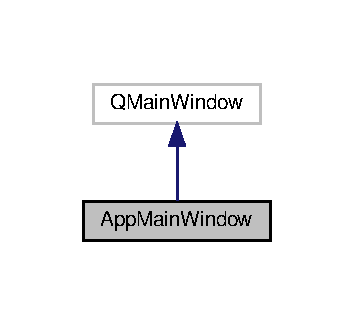
\includegraphics[width=170pt]{classAppMainWindow__inherit__graph}
\end{center}
\end{figure}


Graphe de collaboration de App\+Main\+Window\+:\nopagebreak
\begin{figure}[H]
\begin{center}
\leavevmode
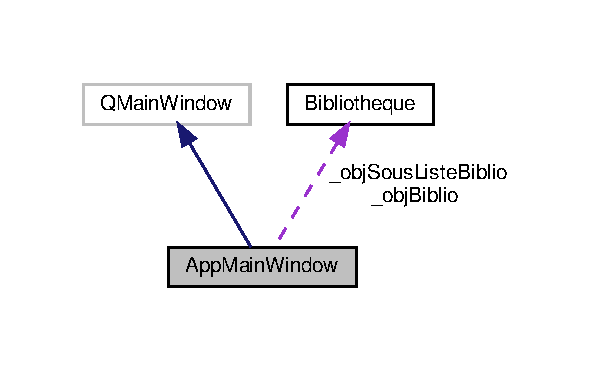
\includegraphics[width=284pt]{classAppMainWindow__coll__graph}
\end{center}
\end{figure}
\subsection*{Fonctions membres publiques}
\begin{DoxyCompactItemize}
\item 
\mbox{\Hypertarget{classAppMainWindow_a80c892efaa500c1e07057923edc81839}\label{classAppMainWindow_a80c892efaa500c1e07057923edc81839}} 
{\bfseries App\+Main\+Window} (Q\+Widget $\ast$parent=0)
\end{DoxyCompactItemize}
\subsection*{Connecteurs privés}
\begin{DoxyCompactItemize}
\item 
\mbox{\Hypertarget{classAppMainWindow_adedddb04ee07d7d8099ee92d70194cd2}\label{classAppMainWindow_adedddb04ee07d7d8099ee92d70194cd2}} 
void \hyperlink{classAppMainWindow_adedddb04ee07d7d8099ee92d70194cd2}{on\+\_\+push\+Button\+Identifier\+\_\+clicked} ()
\begin{DoxyCompactList}\small\item\em on\+\_\+push\+Button\+Identifier\+\_\+clicked \end{DoxyCompactList}\item 
\mbox{\Hypertarget{classAppMainWindow_a55feb1b5e485c1b3a46c2426edf64b4e}\label{classAppMainWindow_a55feb1b5e485c1b3a46c2426edf64b4e}} 
void \hyperlink{classAppMainWindow_a55feb1b5e485c1b3a46c2426edf64b4e}{on\+\_\+push\+Button\+Quitter\+\_\+clicked} ()
\begin{DoxyCompactList}\small\item\em on\+\_\+push\+Button\+Quitter\+\_\+clicked \end{DoxyCompactList}\item 
\mbox{\Hypertarget{classAppMainWindow_a807f1d4b6f2376f4fae0757b8ae17934}\label{classAppMainWindow_a807f1d4b6f2376f4fae0757b8ae17934}} 
void \hyperlink{classAppMainWindow_a807f1d4b6f2376f4fae0757b8ae17934}{on\+\_\+push\+Button\+Charger\+Biblio\+\_\+clicked} ()
\begin{DoxyCompactList}\small\item\em on\+\_\+push\+Button\+Charger\+Biblio\+\_\+clicked \end{DoxyCompactList}\item 
\mbox{\Hypertarget{classAppMainWindow_aaabff27d6afcec8f01dd07b0c3569c53}\label{classAppMainWindow_aaabff27d6afcec8f01dd07b0c3569c53}} 
void \hyperlink{classAppMainWindow_aaabff27d6afcec8f01dd07b0c3569c53}{on\+\_\+push\+Button\+Retour\+Identification\+\_\+clicked} ()
\begin{DoxyCompactList}\small\item\em on\+\_\+push\+Button\+Retour\+Identification\+\_\+clicked \end{DoxyCompactList}\item 
\mbox{\Hypertarget{classAppMainWindow_af642437ed056c378f1bd23afdf57dd46}\label{classAppMainWindow_af642437ed056c378f1bd23afdf57dd46}} 
void \hyperlink{classAppMainWindow_af642437ed056c378f1bd23afdf57dd46}{on\+\_\+table\+Biblio\+Row\+Clicked} (int, int)
\begin{DoxyCompactList}\small\item\em on\+\_\+table\+Biblio\+Row\+Clicked \end{DoxyCompactList}\item 
\mbox{\Hypertarget{classAppMainWindow_abdc070ca216fd50485b42d8b5634c2cd}\label{classAppMainWindow_abdc070ca216fd50485b42d8b5634c2cd}} 
void \hyperlink{classAppMainWindow_abdc070ca216fd50485b42d8b5634c2cd}{on\+\_\+push\+Button\+Sauvegarder\+\_\+clicked} ()
\begin{DoxyCompactList}\small\item\em on\+\_\+push\+Button\+Sauvegarder\+\_\+clicked \end{DoxyCompactList}\item 
\mbox{\Hypertarget{classAppMainWindow_a63b12959410f1c4cdcf2ec429d0757ac}\label{classAppMainWindow_a63b12959410f1c4cdcf2ec429d0757ac}} 
void \hyperlink{classAppMainWindow_a63b12959410f1c4cdcf2ec429d0757ac}{on\+\_\+push\+Button\+Supprimer\+Image\+\_\+clicked} ()
\begin{DoxyCompactList}\small\item\em on\+\_\+push\+Button\+Supprimer\+Image\+\_\+clicked \end{DoxyCompactList}\item 
\mbox{\Hypertarget{classAppMainWindow_a48ca3eef57a64ce991111e6d06995711}\label{classAppMainWindow_a48ca3eef57a64ce991111e6d06995711}} 
void \hyperlink{classAppMainWindow_a48ca3eef57a64ce991111e6d06995711}{on\+\_\+push\+Button\+Retour\+Menu\+Principal\+\_\+clicked} ()
\begin{DoxyCompactList}\small\item\em on\+\_\+push\+Button\+Retour\+Menu\+Principal\+\_\+clicked \end{DoxyCompactList}\item 
\mbox{\Hypertarget{classAppMainWindow_a613b1fa991ada095afd521f8ec1049b8}\label{classAppMainWindow_a613b1fa991ada095afd521f8ec1049b8}} 
void \hyperlink{classAppMainWindow_a613b1fa991ada095afd521f8ec1049b8}{on\+\_\+line\+Edit\+Mdp\+\_\+return\+Pressed} ()
\begin{DoxyCompactList}\small\item\em on\+\_\+line\+Edit\+Mdp\+\_\+return\+Pressed \end{DoxyCompactList}\item 
\mbox{\Hypertarget{classAppMainWindow_a8aaafc24ce68ff58b2c96177b237db52}\label{classAppMainWindow_a8aaafc24ce68ff58b2c96177b237db52}} 
void \hyperlink{classAppMainWindow_a8aaafc24ce68ff58b2c96177b237db52}{on\+\_\+combo\+Box\+Trier\+Index\+Changed} (int)
\begin{DoxyCompactList}\small\item\em on\+\_\+combo\+Box\+Trier\+Index\+Changed \end{DoxyCompactList}\item 
\mbox{\Hypertarget{classAppMainWindow_aa3aa7020d15253d302bab9b173c39292}\label{classAppMainWindow_aa3aa7020d15253d302bab9b173c39292}} 
void \hyperlink{classAppMainWindow_aa3aa7020d15253d302bab9b173c39292}{on\+\_\+combo\+Box\+Critere\+Cout\+Index\+Changed} (int)
\begin{DoxyCompactList}\small\item\em on\+\_\+combo\+Box\+Critere\+Cout\+Index\+Changed \end{DoxyCompactList}\item 
\mbox{\Hypertarget{classAppMainWindow_ad9bea95541f32cc85642a4f0434cc2c0}\label{classAppMainWindow_ad9bea95541f32cc85642a4f0434cc2c0}} 
void \hyperlink{classAppMainWindow_ad9bea95541f32cc85642a4f0434cc2c0}{on\+\_\+combo\+Box\+Critere\+Date\+Ajout\+Index\+Changed} (int)
\begin{DoxyCompactList}\small\item\em on\+\_\+combo\+Box\+Critere\+Date\+Ajout\+Index\+Changed \end{DoxyCompactList}\item 
\mbox{\Hypertarget{classAppMainWindow_a3d480e06ffddc52d13b6f59364edf4d6}\label{classAppMainWindow_a3d480e06ffddc52d13b6f59364edf4d6}} 
void \hyperlink{classAppMainWindow_a3d480e06ffddc52d13b6f59364edf4d6}{on\+\_\+push\+Button\+Ajouter\+Image\+\_\+clicked} ()
\begin{DoxyCompactList}\small\item\em on\+\_\+push\+Button\+Ajouter\+Image\+\_\+clicked \end{DoxyCompactList}\item 
\mbox{\Hypertarget{classAppMainWindow_a8213943a9db983045e1f250c4ae24409}\label{classAppMainWindow_a8213943a9db983045e1f250c4ae24409}} 
void \hyperlink{classAppMainWindow_a8213943a9db983045e1f250c4ae24409}{on\+\_\+push\+Button\+Ajout\+Image\+Annuler\+\_\+clicked} ()
\begin{DoxyCompactList}\small\item\em on\+\_\+push\+Button\+Ajout\+Image\+Annuler\+\_\+clicked \end{DoxyCompactList}\item 
\mbox{\Hypertarget{classAppMainWindow_a3615ac5567a585a4dcee7966bf06c6ae}\label{classAppMainWindow_a3615ac5567a585a4dcee7966bf06c6ae}} 
void \hyperlink{classAppMainWindow_a3615ac5567a585a4dcee7966bf06c6ae}{on\+\_\+push\+Button\+Ajout\+Image\+Ajouter\+\_\+clicked} ()
\begin{DoxyCompactList}\small\item\em on\+\_\+push\+Button\+Ajout\+Image\+Ajouter\+\_\+clicked \end{DoxyCompactList}\item 
\mbox{\Hypertarget{classAppMainWindow_a9a3339b93e5dc22b925092f771c3079b}\label{classAppMainWindow_a9a3339b93e5dc22b925092f771c3079b}} 
void \hyperlink{classAppMainWindow_a9a3339b93e5dc22b925092f771c3079b}{on\+\_\+push\+Button\+Creer\+Biblio\+\_\+clicked} ()
\begin{DoxyCompactList}\small\item\em on\+\_\+push\+Button\+Creer\+Biblio\+\_\+clicked \end{DoxyCompactList}\item 
\mbox{\Hypertarget{classAppMainWindow_a15481935096c0f5b09cdb611fc9cde2a}\label{classAppMainWindow_a15481935096c0f5b09cdb611fc9cde2a}} 
void \hyperlink{classAppMainWindow_a15481935096c0f5b09cdb611fc9cde2a}{on\+\_\+push\+Button\+Sauvegarder\+Sous\+Liste\+\_\+clicked} ()
\begin{DoxyCompactList}\small\item\em on\+\_\+push\+Button\+Sauvegarder\+Sous\+Liste\+\_\+clicked \end{DoxyCompactList}\item 
\mbox{\Hypertarget{classAppMainWindow_aab451b9f2216824cb996f5b0df9a57ac}\label{classAppMainWindow_aab451b9f2216824cb996f5b0df9a57ac}} 
void \hyperlink{classAppMainWindow_aab451b9f2216824cb996f5b0df9a57ac}{on\+\_\+push\+Button\+Ouvrir\+Image\+\_\+clicked} ()
\begin{DoxyCompactList}\small\item\em on\+\_\+push\+Button\+Ouvrir\+Image\+\_\+clicked \end{DoxyCompactList}\item 
\mbox{\Hypertarget{classAppMainWindow_af31732baab71f621b62bf06df6a7e8bf}\label{classAppMainWindow_af31732baab71f621b62bf06df6a7e8bf}} 
void \hyperlink{classAppMainWindow_af31732baab71f621b62bf06df6a7e8bf}{on\+\_\+push\+Button\+Retour\+Menu\+Modification\+Image\+\_\+clicked} ()
\begin{DoxyCompactList}\small\item\em on\+\_\+push\+Button\+Retour\+Menu\+Modification\+Image\+\_\+clicked \end{DoxyCompactList}\item 
\mbox{\Hypertarget{classAppMainWindow_a788925d89b1ddd65bd925bbe5edd228d}\label{classAppMainWindow_a788925d89b1ddd65bd925bbe5edd228d}} 
void \hyperlink{classAppMainWindow_a788925d89b1ddd65bd925bbe5edd228d}{on\+\_\+double\+Spin\+Box\+Min\+\_\+value\+Changed} (double)
\begin{DoxyCompactList}\small\item\em on\+\_\+double\+Spin\+Box\+Min\+\_\+value\+Changed \end{DoxyCompactList}\item 
\mbox{\Hypertarget{classAppMainWindow_a937503d2539b01093ee2c3479918bf7f}\label{classAppMainWindow_a937503d2539b01093ee2c3479918bf7f}} 
void \hyperlink{classAppMainWindow_a937503d2539b01093ee2c3479918bf7f}{on\+\_\+double\+Spin\+Box\+Max\+\_\+value\+Changed} (double)
\begin{DoxyCompactList}\small\item\em on\+\_\+double\+Spin\+Box\+Max\+\_\+value\+Changed \end{DoxyCompactList}\item 
\mbox{\Hypertarget{classAppMainWindow_a3465793b22d26803be33b64758933fb7}\label{classAppMainWindow_a3465793b22d26803be33b64758933fb7}} 
void \hyperlink{classAppMainWindow_a3465793b22d26803be33b64758933fb7}{on\+\_\+horizontal\+Slider\+\_\+agrandissement\+Non\+Modifiable\+\_\+value\+Changed} (int)
\begin{DoxyCompactList}\small\item\em on\+\_\+horizontal\+Slider\+\_\+agrandissement\+Non\+Modifiable\+\_\+value\+Changed \end{DoxyCompactList}\item 
\mbox{\Hypertarget{classAppMainWindow_ab8bab04abb5d76bfffbc5c6d468ee981}\label{classAppMainWindow_ab8bab04abb5d76bfffbc5c6d468ee981}} 
void \hyperlink{classAppMainWindow_ab8bab04abb5d76bfffbc5c6d468ee981}{on\+\_\+push\+Button\+\_\+modifier\+\_\+clicked} ()
\begin{DoxyCompactList}\small\item\em on\+\_\+push\+Button\+\_\+modifier\+\_\+clicked \end{DoxyCompactList}\item 
\mbox{\Hypertarget{classAppMainWindow_a49ba69820f7ed19e7dd245aa60479fee}\label{classAppMainWindow_a49ba69820f7ed19e7dd245aa60479fee}} 
void \hyperlink{classAppMainWindow_a49ba69820f7ed19e7dd245aa60479fee}{on\+\_\+horizontal\+Slider\+\_\+agrandissement\+\_\+value\+Changed} (int)
\begin{DoxyCompactList}\small\item\em on\+\_\+horizontal\+Slider\+\_\+agrandissement\+\_\+value\+Changed \end{DoxyCompactList}\item 
\mbox{\Hypertarget{classAppMainWindow_a094e49f72edd2a6b229f14aaff268baa}\label{classAppMainWindow_a094e49f72edd2a6b229f14aaff268baa}} 
void \hyperlink{classAppMainWindow_a094e49f72edd2a6b229f14aaff268baa}{on\+\_\+push\+Button\+\_\+traitement\+Image\+\_\+clicked} ()
\begin{DoxyCompactList}\small\item\em on\+\_\+push\+Button\+\_\+traitement\+Image\+\_\+clicked \end{DoxyCompactList}\item 
\mbox{\Hypertarget{classAppMainWindow_ad88e547ca3b09758ee7695b936bcf8e9}\label{classAppMainWindow_ad88e547ca3b09758ee7695b936bcf8e9}} 
void \hyperlink{classAppMainWindow_ad88e547ca3b09758ee7695b936bcf8e9}{on\+\_\+push\+Button\+\_\+retour\+\_\+clicked} ()
\begin{DoxyCompactList}\small\item\em on\+\_\+push\+Button\+\_\+retour\+\_\+clicked \end{DoxyCompactList}\item 
\mbox{\Hypertarget{classAppMainWindow_ab89de41267707db6ce2e05d81426ca52}\label{classAppMainWindow_ab89de41267707db6ce2e05d81426ca52}} 
void \hyperlink{classAppMainWindow_ab89de41267707db6ce2e05d81426ca52}{on\+\_\+horizontal\+Slider\+\_\+image\+Originale\+\_\+value\+Changed} (int)
\begin{DoxyCompactList}\small\item\em on\+\_\+horizontal\+Slider\+\_\+image\+Originale\+\_\+value\+Changed \end{DoxyCompactList}\item 
\mbox{\Hypertarget{classAppMainWindow_a93072ed048c9f2787297287aeabcbc5c}\label{classAppMainWindow_a93072ed048c9f2787297287aeabcbc5c}} 
void \hyperlink{classAppMainWindow_a93072ed048c9f2787297287aeabcbc5c}{on\+\_\+horizontal\+Slider\+\_\+image\+Traitee\+\_\+value\+Changed} (int)
\begin{DoxyCompactList}\small\item\em on\+\_\+horizontal\+Slider\+\_\+image\+Traitee\+\_\+value\+Changed \end{DoxyCompactList}\item 
\mbox{\Hypertarget{classAppMainWindow_adff9d30acf6ab3f326244e854539f6c3}\label{classAppMainWindow_adff9d30acf6ab3f326244e854539f6c3}} 
void \hyperlink{classAppMainWindow_adff9d30acf6ab3f326244e854539f6c3}{on\+\_\+push\+Button\+\_\+traitement\+Reinitialiser\+\_\+clicked} ()
\begin{DoxyCompactList}\small\item\em on\+\_\+push\+Button\+\_\+traitement\+Reinitialiser\+\_\+clicked \end{DoxyCompactList}\item 
\mbox{\Hypertarget{classAppMainWindow_a28183f9ca4c7385aed673c258a89d272}\label{classAppMainWindow_a28183f9ca4c7385aed673c258a89d272}} 
void \hyperlink{classAppMainWindow_a28183f9ca4c7385aed673c258a89d272}{on\+\_\+push\+Button\+\_\+traitement\+Appliquer\+\_\+clicked} ()
\begin{DoxyCompactList}\small\item\em on\+\_\+push\+Button\+\_\+traitement\+Appliquer\+\_\+clicked \end{DoxyCompactList}\item 
\mbox{\Hypertarget{classAppMainWindow_a3fb09e5476491ccb373c3142568ea9b0}\label{classAppMainWindow_a3fb09e5476491ccb373c3142568ea9b0}} 
void \hyperlink{classAppMainWindow_a3fb09e5476491ccb373c3142568ea9b0}{on\+\_\+group\+Box\+\_\+correction\+\_\+clicked} ()
\begin{DoxyCompactList}\small\item\em on\+\_\+group\+Box\+\_\+correction\+\_\+clicked \end{DoxyCompactList}\item 
\mbox{\Hypertarget{classAppMainWindow_a1a387398116058b46cf8471ff4074f3d}\label{classAppMainWindow_a1a387398116058b46cf8471ff4074f3d}} 
void \hyperlink{classAppMainWindow_a1a387398116058b46cf8471ff4074f3d}{on\+\_\+radio\+Button\+\_\+luminosite\+\_\+clicked} ()
\begin{DoxyCompactList}\small\item\em on\+\_\+radio\+Button\+\_\+luminosite\+\_\+clicked \end{DoxyCompactList}\item 
\mbox{\Hypertarget{classAppMainWindow_abd9ddc7e5b68c639f077e7b5ae72427b}\label{classAppMainWindow_abd9ddc7e5b68c639f077e7b5ae72427b}} 
void \hyperlink{classAppMainWindow_abd9ddc7e5b68c639f077e7b5ae72427b}{on\+\_\+horizontal\+Slider\+\_\+luminosite\+\_\+value\+Changed} (int)
\begin{DoxyCompactList}\small\item\em on\+\_\+horizontal\+Slider\+\_\+luminosite\+\_\+value\+Changed \end{DoxyCompactList}\item 
\mbox{\Hypertarget{classAppMainWindow_a42e59487ad33350eebc89972af1061a7}\label{classAppMainWindow_a42e59487ad33350eebc89972af1061a7}} 
void \hyperlink{classAppMainWindow_a42e59487ad33350eebc89972af1061a7}{on\+\_\+radio\+Button\+\_\+contraste\+\_\+clicked} ()
\begin{DoxyCompactList}\small\item\em on\+\_\+radio\+Button\+\_\+contraste\+\_\+clicked \end{DoxyCompactList}\item 
\mbox{\Hypertarget{classAppMainWindow_a62da52f18d62803f4ccf6322507b918c}\label{classAppMainWindow_a62da52f18d62803f4ccf6322507b918c}} 
void \hyperlink{classAppMainWindow_a62da52f18d62803f4ccf6322507b918c}{on\+\_\+horizontal\+Slider\+\_\+contraste\+\_\+value\+Changed} (int)
\begin{DoxyCompactList}\small\item\em on\+\_\+horizontal\+Slider\+\_\+contraste\+\_\+value\+Changed \end{DoxyCompactList}\item 
\mbox{\Hypertarget{classAppMainWindow_a92e81ef96a67355118357cb6ab94f0d9}\label{classAppMainWindow_a92e81ef96a67355118357cb6ab94f0d9}} 
void \hyperlink{classAppMainWindow_a92e81ef96a67355118357cb6ab94f0d9}{on\+\_\+radio\+Button\+\_\+ombre\+\_\+clicked} ()
\begin{DoxyCompactList}\small\item\em on\+\_\+radio\+Button\+\_\+ombre\+\_\+clicked \end{DoxyCompactList}\item 
\mbox{\Hypertarget{classAppMainWindow_ae8bdd8fb835d78149e82e6092ef4bb49}\label{classAppMainWindow_ae8bdd8fb835d78149e82e6092ef4bb49}} 
void \hyperlink{classAppMainWindow_ae8bdd8fb835d78149e82e6092ef4bb49}{on\+\_\+horizontal\+Slider\+\_\+ombre\+\_\+value\+Changed} (int)
\begin{DoxyCompactList}\small\item\em on\+\_\+horizontal\+Slider\+\_\+ombre\+\_\+value\+Changed \end{DoxyCompactList}\item 
\mbox{\Hypertarget{classAppMainWindow_af6ea50a2b74e6d9d1142c1505e83f74c}\label{classAppMainWindow_af6ea50a2b74e6d9d1142c1505e83f74c}} 
void \hyperlink{classAppMainWindow_af6ea50a2b74e6d9d1142c1505e83f74c}{on\+\_\+radio\+Button\+\_\+brillance\+\_\+clicked} ()
\begin{DoxyCompactList}\small\item\em on\+\_\+radio\+Button\+\_\+brillance\+\_\+clicked \end{DoxyCompactList}\item 
\mbox{\Hypertarget{classAppMainWindow_a97ec43262c96c703ac380393177c6e11}\label{classAppMainWindow_a97ec43262c96c703ac380393177c6e11}} 
void \hyperlink{classAppMainWindow_a97ec43262c96c703ac380393177c6e11}{on\+\_\+horizontal\+Slider\+\_\+brillance\+\_\+value\+Changed} (int)
\begin{DoxyCompactList}\small\item\em on\+\_\+horizontal\+Slider\+\_\+brillance\+\_\+value\+Changed \end{DoxyCompactList}\item 
\mbox{\Hypertarget{classAppMainWindow_a1a44bb8a30a009b31a310afbd8b6f5d5}\label{classAppMainWindow_a1a44bb8a30a009b31a310afbd8b6f5d5}} 
void \hyperlink{classAppMainWindow_a1a44bb8a30a009b31a310afbd8b6f5d5}{on\+\_\+group\+Box\+\_\+details\+\_\+clicked} ()
\begin{DoxyCompactList}\small\item\em on\+\_\+group\+Box\+\_\+details\+\_\+clicked \end{DoxyCompactList}\item 
\mbox{\Hypertarget{classAppMainWindow_a415ee61f1bad859435161a153ffb5ddd}\label{classAppMainWindow_a415ee61f1bad859435161a153ffb5ddd}} 
void \hyperlink{classAppMainWindow_a415ee61f1bad859435161a153ffb5ddd}{on\+\_\+radio\+Button\+\_\+nettete\+\_\+clicked} ()
\begin{DoxyCompactList}\small\item\em on\+\_\+radio\+Button\+\_\+nettete\+\_\+clicked \end{DoxyCompactList}\item 
\mbox{\Hypertarget{classAppMainWindow_abbf6f7da99ff178646ddae8b6210695a}\label{classAppMainWindow_abbf6f7da99ff178646ddae8b6210695a}} 
void \hyperlink{classAppMainWindow_abbf6f7da99ff178646ddae8b6210695a}{on\+\_\+horizontal\+Slider\+\_\+nettete\+\_\+value\+Changed} (int)
\begin{DoxyCompactList}\small\item\em on\+\_\+horizontal\+Slider\+\_\+nettete\+\_\+value\+Changed \end{DoxyCompactList}\item 
\mbox{\Hypertarget{classAppMainWindow_aaba7dfcc45216efadf523e0e303d1751}\label{classAppMainWindow_aaba7dfcc45216efadf523e0e303d1751}} 
void \hyperlink{classAppMainWindow_aaba7dfcc45216efadf523e0e303d1751}{on\+\_\+radio\+Button\+\_\+bruitage\+\_\+clicked} ()
\begin{DoxyCompactList}\small\item\em on\+\_\+radio\+Button\+\_\+bruitage\+\_\+clicked \end{DoxyCompactList}\item 
\mbox{\Hypertarget{classAppMainWindow_a88a4155c1540115b46a39691e520362b}\label{classAppMainWindow_a88a4155c1540115b46a39691e520362b}} 
void \hyperlink{classAppMainWindow_a88a4155c1540115b46a39691e520362b}{on\+\_\+horizontal\+Slider\+\_\+\+Bruitage\+\_\+value\+Changed} (int)
\begin{DoxyCompactList}\small\item\em on\+\_\+horizontal\+Slider\+\_\+\+Bruitage\+\_\+value\+Changed \end{DoxyCompactList}\item 
\mbox{\Hypertarget{classAppMainWindow_a664a99b0efe59a0281ecca95305b85a1}\label{classAppMainWindow_a664a99b0efe59a0281ecca95305b85a1}} 
void \hyperlink{classAppMainWindow_a664a99b0efe59a0281ecca95305b85a1}{on\+\_\+group\+Box\+\_\+filtres\+\_\+clicked} ()
\begin{DoxyCompactList}\small\item\em on\+\_\+group\+Box\+\_\+filtres\+\_\+clicked \end{DoxyCompactList}\item 
\mbox{\Hypertarget{classAppMainWindow_af2bc6c9054b58823f3a0fa79e4f2ccde}\label{classAppMainWindow_af2bc6c9054b58823f3a0fa79e4f2ccde}} 
void \hyperlink{classAppMainWindow_af2bc6c9054b58823f3a0fa79e4f2ccde}{on\+\_\+radio\+Button\+\_\+originale\+\_\+clicked} ()
\begin{DoxyCompactList}\small\item\em on\+\_\+radio\+Button\+\_\+originale\+\_\+clicked \end{DoxyCompactList}\item 
\mbox{\Hypertarget{classAppMainWindow_a49bda23245ce5b1935669a6a50a22d65}\label{classAppMainWindow_a49bda23245ce5b1935669a6a50a22d65}} 
void \hyperlink{classAppMainWindow_a49bda23245ce5b1935669a6a50a22d65}{on\+\_\+radio\+Button\+\_\+niveau\+Gris\+\_\+clicked} ()
\begin{DoxyCompactList}\small\item\em on\+\_\+radio\+Button\+\_\+niveau\+Gris\+\_\+clicked \end{DoxyCompactList}\item 
\mbox{\Hypertarget{classAppMainWindow_a529f3a819034ca1497ff3d20994dba3c}\label{classAppMainWindow_a529f3a819034ca1497ff3d20994dba3c}} 
void \hyperlink{classAppMainWindow_a529f3a819034ca1497ff3d20994dba3c}{on\+\_\+radio\+Button\+\_\+inversement\+\_\+clicked} ()
\begin{DoxyCompactList}\small\item\em on\+\_\+radio\+Button\+\_\+inversement\+\_\+clicked \end{DoxyCompactList}\item 
\mbox{\Hypertarget{classAppMainWindow_a9e7a5a2b083e8d3c309bbd1beaf14937}\label{classAppMainWindow_a9e7a5a2b083e8d3c309bbd1beaf14937}} 
void \hyperlink{classAppMainWindow_a9e7a5a2b083e8d3c309bbd1beaf14937}{on\+\_\+radio\+Button\+\_\+rouge\+\_\+clicked} ()
\begin{DoxyCompactList}\small\item\em on\+\_\+radio\+Button\+\_\+rouge\+\_\+clicked \end{DoxyCompactList}\item 
\mbox{\Hypertarget{classAppMainWindow_a05d60ab1798f79750d3e76dc0ba72125}\label{classAppMainWindow_a05d60ab1798f79750d3e76dc0ba72125}} 
void \hyperlink{classAppMainWindow_a05d60ab1798f79750d3e76dc0ba72125}{on\+\_\+radio\+Button\+\_\+vert\+\_\+clicked} ()
\begin{DoxyCompactList}\small\item\em on\+\_\+radio\+Button\+\_\+vert\+\_\+clicked \end{DoxyCompactList}\item 
\mbox{\Hypertarget{classAppMainWindow_a13a13abc5a8acf68376e529cf8210d68}\label{classAppMainWindow_a13a13abc5a8acf68376e529cf8210d68}} 
void \hyperlink{classAppMainWindow_a13a13abc5a8acf68376e529cf8210d68}{on\+\_\+radio\+Button\+\_\+bleu\+\_\+clicked} ()
\begin{DoxyCompactList}\small\item\em on\+\_\+radio\+Button\+\_\+bleu\+\_\+clicked \end{DoxyCompactList}\item 
\mbox{\Hypertarget{classAppMainWindow_afeaabe78d568450d2f8a18920d11e0af}\label{classAppMainWindow_afeaabe78d568450d2f8a18920d11e0af}} 
void \hyperlink{classAppMainWindow_afeaabe78d568450d2f8a18920d11e0af}{on\+\_\+radio\+Button\+\_\+jaune\+\_\+clicked} ()
\begin{DoxyCompactList}\small\item\em on\+\_\+radio\+Button\+\_\+jaune\+\_\+clicked \end{DoxyCompactList}\item 
\mbox{\Hypertarget{classAppMainWindow_a6ee4ea2dd658df7860edfb53ccb1c894}\label{classAppMainWindow_a6ee4ea2dd658df7860edfb53ccb1c894}} 
void \hyperlink{classAppMainWindow_a6ee4ea2dd658df7860edfb53ccb1c894}{on\+\_\+radio\+Button\+\_\+cyan\+\_\+clicked} ()
\begin{DoxyCompactList}\small\item\em on\+\_\+radio\+Button\+\_\+cyan\+\_\+clicked \end{DoxyCompactList}\item 
\mbox{\Hypertarget{classAppMainWindow_acc36f02cf06cb0295bd0684c014a5a48}\label{classAppMainWindow_acc36f02cf06cb0295bd0684c014a5a48}} 
void \hyperlink{classAppMainWindow_acc36f02cf06cb0295bd0684c014a5a48}{on\+\_\+radio\+Button\+\_\+sepia\+\_\+clicked} ()
\begin{DoxyCompactList}\small\item\em on\+\_\+radio\+Button\+\_\+sepia\+\_\+clicked \end{DoxyCompactList}\item 
\mbox{\Hypertarget{classAppMainWindow_a785f5e333d62dba43501387794e36f94}\label{classAppMainWindow_a785f5e333d62dba43501387794e36f94}} 
void \hyperlink{classAppMainWindow_a785f5e333d62dba43501387794e36f94}{on\+\_\+radio\+Button\+\_\+magenta\+\_\+clicked} ()
\begin{DoxyCompactList}\small\item\em on\+\_\+radio\+Button\+\_\+magenta\+\_\+clicked \end{DoxyCompactList}\item 
\mbox{\Hypertarget{classAppMainWindow_a17792a2be779a477e8b39f6101934453}\label{classAppMainWindow_a17792a2be779a477e8b39f6101934453}} 
void \hyperlink{classAppMainWindow_a17792a2be779a477e8b39f6101934453}{on\+\_\+radio\+Button\+\_\+rgb\+\_\+clicked} ()
\begin{DoxyCompactList}\small\item\em on\+\_\+radio\+Button\+\_\+rgb\+\_\+clicked \end{DoxyCompactList}\item 
\mbox{\Hypertarget{classAppMainWindow_aa8f659155495c4654b58a81402e15c62}\label{classAppMainWindow_aa8f659155495c4654b58a81402e15c62}} 
void \hyperlink{classAppMainWindow_aa8f659155495c4654b58a81402e15c62}{on\+\_\+group\+Box\+\_\+extraction\+R\+V\+B\+\_\+clicked} ()
\begin{DoxyCompactList}\small\item\em on\+\_\+group\+Box\+\_\+extraction\+R\+V\+B\+\_\+clicked \end{DoxyCompactList}\item 
\mbox{\Hypertarget{classAppMainWindow_a99efb1da0e9cf4ea1e12a43f8aff9402}\label{classAppMainWindow_a99efb1da0e9cf4ea1e12a43f8aff9402}} 
void \hyperlink{classAppMainWindow_a99efb1da0e9cf4ea1e12a43f8aff9402}{on\+\_\+radio\+Button\+\_\+extraction\+R\+\_\+clicked} ()
\begin{DoxyCompactList}\small\item\em on\+\_\+radio\+Button\+\_\+extraction\+R\+\_\+clicked \end{DoxyCompactList}\item 
\mbox{\Hypertarget{classAppMainWindow_a05522b3bbaeab71f9f16db88e5a34ccc}\label{classAppMainWindow_a05522b3bbaeab71f9f16db88e5a34ccc}} 
void \hyperlink{classAppMainWindow_a05522b3bbaeab71f9f16db88e5a34ccc}{on\+\_\+radio\+Button\+\_\+extraction\+V\+\_\+clicked} ()
\begin{DoxyCompactList}\small\item\em on\+\_\+radio\+Button\+\_\+extraction\+V\+\_\+clicked \end{DoxyCompactList}\item 
\mbox{\Hypertarget{classAppMainWindow_a060bb63eea429b322b274ab70649cc47}\label{classAppMainWindow_a060bb63eea429b322b274ab70649cc47}} 
void \hyperlink{classAppMainWindow_a060bb63eea429b322b274ab70649cc47}{on\+\_\+radio\+Button\+\_\+extraction\+B\+\_\+clicked} ()
\begin{DoxyCompactList}\small\item\em on\+\_\+radio\+Button\+\_\+extraction\+B\+\_\+clicked \end{DoxyCompactList}\item 
\mbox{\Hypertarget{classAppMainWindow_af2747bc08aa9f5256c7b3193571cbb34}\label{classAppMainWindow_af2747bc08aa9f5256c7b3193571cbb34}} 
void \hyperlink{classAppMainWindow_af2747bc08aa9f5256c7b3193571cbb34}{on\+\_\+group\+Box\+\_\+seuillage\+Segmentation\+\_\+clicked} ()
\begin{DoxyCompactList}\small\item\em on\+\_\+group\+Box\+\_\+seuillage\+Segmentation\+\_\+clicked \end{DoxyCompactList}\item 
\mbox{\Hypertarget{classAppMainWindow_a2ea6682a925bd79c362823e731f2382f}\label{classAppMainWindow_a2ea6682a925bd79c362823e731f2382f}} 
void \hyperlink{classAppMainWindow_a2ea6682a925bd79c362823e731f2382f}{on\+\_\+radio\+Button\+\_\+seuillage\+\_\+clicked} ()
\begin{DoxyCompactList}\small\item\em on\+\_\+radio\+Button\+\_\+seuillage\+\_\+clicked \end{DoxyCompactList}\item 
\mbox{\Hypertarget{classAppMainWindow_a4bc1c1b0ca46ffd7bd26141aa6f130dc}\label{classAppMainWindow_a4bc1c1b0ca46ffd7bd26141aa6f130dc}} 
void \hyperlink{classAppMainWindow_a4bc1c1b0ca46ffd7bd26141aa6f130dc}{on\+\_\+radio\+Button\+\_\+segmentation\+\_\+clicked} ()
\begin{DoxyCompactList}\small\item\em on\+\_\+radio\+Button\+\_\+segmentation\+\_\+clicked \end{DoxyCompactList}\item 
\mbox{\Hypertarget{classAppMainWindow_a578a5ab65f2b64536d6d7d7588d603c1}\label{classAppMainWindow_a578a5ab65f2b64536d6d7d7588d603c1}} 
void \hyperlink{classAppMainWindow_a578a5ab65f2b64536d6d7d7588d603c1}{on\+\_\+radio\+Button\+\_\+seuillage\+Simple\+\_\+clicked} ()
\begin{DoxyCompactList}\small\item\em on\+\_\+radio\+Button\+\_\+seuillage\+Simple\+\_\+clicked \end{DoxyCompactList}\item 
\mbox{\Hypertarget{classAppMainWindow_ac201450dfce689485b0047efe6a73546}\label{classAppMainWindow_ac201450dfce689485b0047efe6a73546}} 
void \hyperlink{classAppMainWindow_ac201450dfce689485b0047efe6a73546}{on\+\_\+radio\+Button\+\_\+seuillage\+Hysteresis\+\_\+clicked} ()
\begin{DoxyCompactList}\small\item\em on\+\_\+radio\+Button\+\_\+seuillage\+Hysteresis\+\_\+clicked \end{DoxyCompactList}\item 
\mbox{\Hypertarget{classAppMainWindow_a3a5d3c2a8d12dd247b784efb98d11cb1}\label{classAppMainWindow_a3a5d3c2a8d12dd247b784efb98d11cb1}} 
void \hyperlink{classAppMainWindow_a3a5d3c2a8d12dd247b784efb98d11cb1}{on\+\_\+vertical\+Slider\+\_\+seuil\+Bas\+R\+\_\+2\+\_\+value\+Changed} (int)
\begin{DoxyCompactList}\small\item\em on\+\_\+vertical\+Slider\+\_\+seuil\+Bas\+R\+\_\+2\+\_\+value\+Changed \end{DoxyCompactList}\item 
\mbox{\Hypertarget{classAppMainWindow_a2f5e9d42a0d5f4c716320098091110b1}\label{classAppMainWindow_a2f5e9d42a0d5f4c716320098091110b1}} 
void \hyperlink{classAppMainWindow_a2f5e9d42a0d5f4c716320098091110b1}{on\+\_\+vertical\+Slider\+\_\+seuil\+Bas\+V\+\_\+2\+\_\+value\+Changed} (int)
\begin{DoxyCompactList}\small\item\em on\+\_\+vertical\+Slider\+\_\+seuil\+Bas\+V\+\_\+2\+\_\+value\+Changed \end{DoxyCompactList}\item 
\mbox{\Hypertarget{classAppMainWindow_a79462b0c856af1af6321ee51d3461610}\label{classAppMainWindow_a79462b0c856af1af6321ee51d3461610}} 
void \hyperlink{classAppMainWindow_a79462b0c856af1af6321ee51d3461610}{on\+\_\+vertical\+Slider\+\_\+seuil\+Bas\+B\+\_\+2\+\_\+value\+Changed} (int)
\begin{DoxyCompactList}\small\item\em on\+\_\+vertical\+Slider\+\_\+seuil\+Bas\+B\+\_\+2\+\_\+value\+Changed \end{DoxyCompactList}\item 
\mbox{\Hypertarget{classAppMainWindow_a2af3d490aa4ea2e233019f0730ac3645}\label{classAppMainWindow_a2af3d490aa4ea2e233019f0730ac3645}} 
void \hyperlink{classAppMainWindow_a2af3d490aa4ea2e233019f0730ac3645}{on\+\_\+vertical\+Slider\+\_\+seuil\+Haut\+R\+\_\+2\+\_\+value\+Changed} (int)
\begin{DoxyCompactList}\small\item\em on\+\_\+vertical\+Slider\+\_\+seuil\+Haut\+R\+\_\+2\+\_\+value\+Changed \end{DoxyCompactList}\item 
\mbox{\Hypertarget{classAppMainWindow_a59a345a43be67123c4c665d9a063fa49}\label{classAppMainWindow_a59a345a43be67123c4c665d9a063fa49}} 
void \hyperlink{classAppMainWindow_a59a345a43be67123c4c665d9a063fa49}{on\+\_\+vertical\+Slider\+\_\+seuil\+Haut\+V\+\_\+2\+\_\+value\+Changed} (int)
\begin{DoxyCompactList}\small\item\em on\+\_\+vertical\+Slider\+\_\+seuil\+Haut\+V\+\_\+2\+\_\+value\+Changed \end{DoxyCompactList}\item 
\mbox{\Hypertarget{classAppMainWindow_ae8a4edfe036f0147ce8d17f538f83940}\label{classAppMainWindow_ae8a4edfe036f0147ce8d17f538f83940}} 
void \hyperlink{classAppMainWindow_ae8a4edfe036f0147ce8d17f538f83940}{on\+\_\+vertical\+Slider\+\_\+seuil\+Haut\+B\+\_\+2\+\_\+value\+Changed} (int)
\begin{DoxyCompactList}\small\item\em on\+\_\+vertical\+Slider\+\_\+seuil\+Haut\+B\+\_\+2\+\_\+value\+Changed \end{DoxyCompactList}\item 
\mbox{\Hypertarget{classAppMainWindow_a1d28822195b9844712f8bb2f519d293e}\label{classAppMainWindow_a1d28822195b9844712f8bb2f519d293e}} 
void \hyperlink{classAppMainWindow_a1d28822195b9844712f8bb2f519d293e}{on\+\_\+push\+Button\+\_\+seuil\+Bas\+R\+\_\+clicked} ()
\begin{DoxyCompactList}\small\item\em on\+\_\+push\+Button\+\_\+seuil\+Bas\+R\+\_\+clicked \end{DoxyCompactList}\item 
\mbox{\Hypertarget{classAppMainWindow_ac3546f29e76445f9828b261114784d11}\label{classAppMainWindow_ac3546f29e76445f9828b261114784d11}} 
void \hyperlink{classAppMainWindow_ac3546f29e76445f9828b261114784d11}{on\+\_\+push\+Button\+\_\+seuil\+Bas\+V\+\_\+clicked} ()
\begin{DoxyCompactList}\small\item\em on\+\_\+push\+Button\+\_\+seuil\+Bas\+V\+\_\+clicked \end{DoxyCompactList}\item 
\mbox{\Hypertarget{classAppMainWindow_a439ed3f28e156af83fd33534bb798e0c}\label{classAppMainWindow_a439ed3f28e156af83fd33534bb798e0c}} 
void \hyperlink{classAppMainWindow_a439ed3f28e156af83fd33534bb798e0c}{on\+\_\+push\+Button\+\_\+seuil\+Bas\+B\+\_\+clicked} ()
\begin{DoxyCompactList}\small\item\em on\+\_\+push\+Button\+\_\+seuil\+Bas\+B\+\_\+clicked \end{DoxyCompactList}\item 
\mbox{\Hypertarget{classAppMainWindow_a9ae74377e5e195074f3f101e911fdc77}\label{classAppMainWindow_a9ae74377e5e195074f3f101e911fdc77}} 
void \hyperlink{classAppMainWindow_a9ae74377e5e195074f3f101e911fdc77}{on\+\_\+push\+Button\+\_\+seuil\+Haut\+R\+\_\+clicked} ()
\begin{DoxyCompactList}\small\item\em on\+\_\+push\+Button\+\_\+seuil\+Haut\+R\+\_\+clicked \end{DoxyCompactList}\item 
\mbox{\Hypertarget{classAppMainWindow_a5b525c78560d55fc6f235988eee3c9b3}\label{classAppMainWindow_a5b525c78560d55fc6f235988eee3c9b3}} 
void \hyperlink{classAppMainWindow_a5b525c78560d55fc6f235988eee3c9b3}{on\+\_\+push\+Button\+\_\+seuil\+Haut\+V\+\_\+clicked} ()
\begin{DoxyCompactList}\small\item\em on\+\_\+push\+Button\+\_\+seuil\+Haut\+V\+\_\+clicked \end{DoxyCompactList}\item 
\mbox{\Hypertarget{classAppMainWindow_aeea9ea0fbe9ea4252256ae6a679dd7c9}\label{classAppMainWindow_aeea9ea0fbe9ea4252256ae6a679dd7c9}} 
void \hyperlink{classAppMainWindow_aeea9ea0fbe9ea4252256ae6a679dd7c9}{on\+\_\+push\+Button\+\_\+seuil\+Haut\+B\+\_\+clicked} ()
\begin{DoxyCompactList}\small\item\em on\+\_\+push\+Button\+\_\+seuil\+Haut\+B\+\_\+clicked \end{DoxyCompactList}\item 
\mbox{\Hypertarget{classAppMainWindow_a657d4bc284189492b7fbe505dcc207ff}\label{classAppMainWindow_a657d4bc284189492b7fbe505dcc207ff}} 
void \hyperlink{classAppMainWindow_a657d4bc284189492b7fbe505dcc207ff}{on\+\_\+group\+Box\+\_\+contours\+\_\+clicked} ()
\begin{DoxyCompactList}\small\item\em on\+\_\+group\+Box\+\_\+contours\+\_\+clicked \end{DoxyCompactList}\item 
\mbox{\Hypertarget{classAppMainWindow_a84157a1e5e8fac17f37c6c2806ee7795}\label{classAppMainWindow_a84157a1e5e8fac17f37c6c2806ee7795}} 
void \hyperlink{classAppMainWindow_a84157a1e5e8fac17f37c6c2806ee7795}{on\+\_\+radio\+Button\+\_\+contours\+Gradient\+\_\+clicked} ()
\begin{DoxyCompactList}\small\item\em on\+\_\+radio\+Button\+\_\+contours\+Gradient\+\_\+clicked \end{DoxyCompactList}\item 
\mbox{\Hypertarget{classAppMainWindow_a5d0c70fd7f4d6ae9f59b75b235c6e059}\label{classAppMainWindow_a5d0c70fd7f4d6ae9f59b75b235c6e059}} 
void \hyperlink{classAppMainWindow_a5d0c70fd7f4d6ae9f59b75b235c6e059}{on\+\_\+radio\+Button\+\_\+contours\+Laplacien\+\_\+clicked} ()
\begin{DoxyCompactList}\small\item\em on\+\_\+radio\+Button\+\_\+contours\+Laplacien\+\_\+clicked \end{DoxyCompactList}\item 
\mbox{\Hypertarget{classAppMainWindow_a9f2d7bc14684fb1477a057e43ad433fb}\label{classAppMainWindow_a9f2d7bc14684fb1477a057e43ad433fb}} 
void \hyperlink{classAppMainWindow_a9f2d7bc14684fb1477a057e43ad433fb}{on\+\_\+group\+Box\+\_\+resolution\+Quantification\+\_\+clicked} ()
\begin{DoxyCompactList}\small\item\em on\+\_\+group\+Box\+\_\+resolution\+Quantification\+\_\+clicked \end{DoxyCompactList}\item 
\mbox{\Hypertarget{classAppMainWindow_a3d15f22450268932f0a9b55eb7f22fc8}\label{classAppMainWindow_a3d15f22450268932f0a9b55eb7f22fc8}} 
void \hyperlink{classAppMainWindow_a3d15f22450268932f0a9b55eb7f22fc8}{on\+\_\+radio\+Button\+\_\+resolution\+\_\+clicked} ()
\begin{DoxyCompactList}\small\item\em on\+\_\+radio\+Button\+\_\+resolution\+\_\+clicked \end{DoxyCompactList}\item 
\mbox{\Hypertarget{classAppMainWindow_acb52aa1b30dc79877f8fcff2df19c847}\label{classAppMainWindow_acb52aa1b30dc79877f8fcff2df19c847}} 
void \hyperlink{classAppMainWindow_acb52aa1b30dc79877f8fcff2df19c847}{on\+\_\+radio\+Button\+\_\+\+P\+P\+P\+\_\+clicked} ()
\begin{DoxyCompactList}\small\item\em on\+\_\+radio\+Button\+\_\+\+P\+P\+P\+\_\+clicked \end{DoxyCompactList}\item 
\mbox{\Hypertarget{classAppMainWindow_a86c706b829e1d8bc128c9ce376d80e34}\label{classAppMainWindow_a86c706b829e1d8bc128c9ce376d80e34}} 
void \hyperlink{classAppMainWindow_a86c706b829e1d8bc128c9ce376d80e34}{on\+\_\+radio\+Button\+\_\+bipolaire\+\_\+clicked} ()
\begin{DoxyCompactList}\small\item\em on\+\_\+radio\+Button\+\_\+bipolaire\+\_\+clicked \end{DoxyCompactList}\item 
void \hyperlink{classAppMainWindow_a6e8ec3bc33ddf2ccfb66ac9f2bdea798}{on\+\_\+horizontal\+Slider\+\_\+resolution\+\_\+value\+Changed} (int value)
\begin{DoxyCompactList}\small\item\em on\+\_\+horizontal\+Slider\+\_\+resolution\+\_\+value\+Changed \end{DoxyCompactList}\item 
\mbox{\Hypertarget{classAppMainWindow_af4275338b582b00bb35f226a30eac478}\label{classAppMainWindow_af4275338b582b00bb35f226a30eac478}} 
void \hyperlink{classAppMainWindow_af4275338b582b00bb35f226a30eac478}{on\+\_\+radio\+Button\+\_\+quantification\+\_\+clicked} ()
\begin{DoxyCompactList}\small\item\em on\+\_\+radio\+Button\+\_\+quantification\+\_\+clicked \end{DoxyCompactList}\item 
void \hyperlink{classAppMainWindow_a7b6f24303c07e1b41425bc08976a6d93}{on\+\_\+horizontal\+Slider\+\_\+quantification\+\_\+value\+Changed} (int value)
\begin{DoxyCompactList}\small\item\em on\+\_\+horizontal\+Slider\+\_\+quantification\+\_\+value\+Changed \end{DoxyCompactList}\item 
\mbox{\Hypertarget{classAppMainWindow_a2ea10df6c5b039ddc398967690bc5436}\label{classAppMainWindow_a2ea10df6c5b039ddc398967690bc5436}} 
void \hyperlink{classAppMainWindow_a2ea10df6c5b039ddc398967690bc5436}{on\+\_\+group\+Box\+\_\+debruitage\+\_\+clicked} ()
\begin{DoxyCompactList}\small\item\em on\+\_\+group\+Box\+\_\+debruitage\+\_\+clicked \end{DoxyCompactList}\item 
\mbox{\Hypertarget{classAppMainWindow_a9ae8a53aff8676113c49517bae7ba5d2}\label{classAppMainWindow_a9ae8a53aff8676113c49517bae7ba5d2}} 
void \hyperlink{classAppMainWindow_a9ae8a53aff8676113c49517bae7ba5d2}{on\+\_\+radio\+Button\+\_\+moyenneur\+\_\+clicked} ()
\begin{DoxyCompactList}\small\item\em on\+\_\+radio\+Button\+\_\+moyenneur\+\_\+clicked \end{DoxyCompactList}\item 
\mbox{\Hypertarget{classAppMainWindow_aee4cb01973a657803e2d24bfb0a882c2}\label{classAppMainWindow_aee4cb01973a657803e2d24bfb0a882c2}} 
void \hyperlink{classAppMainWindow_aee4cb01973a657803e2d24bfb0a882c2}{on\+\_\+radio\+Button\+\_\+gaussien\+\_\+clicked} ()
\begin{DoxyCompactList}\small\item\em on\+\_\+radio\+Button\+\_\+gaussien\+\_\+clicked \end{DoxyCompactList}\item 
\mbox{\Hypertarget{classAppMainWindow_a8034e487bc2d6f95861fc8b2dd5f46aa}\label{classAppMainWindow_a8034e487bc2d6f95861fc8b2dd5f46aa}} 
void \hyperlink{classAppMainWindow_a8034e487bc2d6f95861fc8b2dd5f46aa}{on\+\_\+radio\+Button\+\_\+median\+\_\+clicked} ()
\begin{DoxyCompactList}\small\item\em on\+\_\+radio\+Button\+\_\+median\+\_\+clicked \end{DoxyCompactList}\item 
\mbox{\Hypertarget{classAppMainWindow_a2d5a87a6dc114994d028e72bb26edf3f}\label{classAppMainWindow_a2d5a87a6dc114994d028e72bb26edf3f}} 
void \hyperlink{classAppMainWindow_a2d5a87a6dc114994d028e72bb26edf3f}{on\+\_\+radio\+Button\+\_\+kuwahara\+\_\+clicked} ()
\begin{DoxyCompactList}\small\item\em on\+\_\+radio\+Button\+\_\+kuwahara\+\_\+clicked \end{DoxyCompactList}\item 
\mbox{\Hypertarget{classAppMainWindow_a56a76ba2077a34598d47c6a937da0599}\label{classAppMainWindow_a56a76ba2077a34598d47c6a937da0599}} 
void \hyperlink{classAppMainWindow_a56a76ba2077a34598d47c6a937da0599}{on\+\_\+group\+Box\+\_\+couleur\+\_\+clicked} ()
\begin{DoxyCompactList}\small\item\em on\+\_\+group\+Box\+\_\+couleur\+\_\+clicked \end{DoxyCompactList}\item 
\mbox{\Hypertarget{classAppMainWindow_ae23e8ea7cc17d595db0d1b43329b646c}\label{classAppMainWindow_ae23e8ea7cc17d595db0d1b43329b646c}} 
void \hyperlink{classAppMainWindow_ae23e8ea7cc17d595db0d1b43329b646c}{on\+\_\+radio\+Button\+\_\+temperature\+\_\+clicked} ()
\begin{DoxyCompactList}\small\item\em on\+\_\+radio\+Button\+\_\+temperature\+\_\+clicked \end{DoxyCompactList}\item 
void \hyperlink{classAppMainWindow_a500aa992a36991cbc4cd6a1fe39bd2ff}{on\+\_\+horizontal\+Slider\+\_\+temperature\+\_\+value\+Changed} (int value)
\begin{DoxyCompactList}\small\item\em on\+\_\+horizontal\+Slider\+\_\+temperature\+\_\+value\+Changed \end{DoxyCompactList}\item 
\mbox{\Hypertarget{classAppMainWindow_a182a51eaf4803bb691d951ffb603b9a2}\label{classAppMainWindow_a182a51eaf4803bb691d951ffb603b9a2}} 
void \hyperlink{classAppMainWindow_a182a51eaf4803bb691d951ffb603b9a2}{on\+\_\+radio\+Button\+\_\+vividite\+\_\+clicked} ()
\begin{DoxyCompactList}\small\item\em on\+\_\+radio\+Button\+\_\+vividite\+\_\+clicked \end{DoxyCompactList}\item 
void \hyperlink{classAppMainWindow_a0de20d498ac66da8fde5776c81b28a2d}{on\+\_\+horizontal\+Slider\+\_\+vividite\+\_\+value\+Changed} (int value)
\begin{DoxyCompactList}\small\item\em on\+\_\+horizontal\+Slider\+\_\+vividite\+\_\+value\+Changed \end{DoxyCompactList}\item 
\mbox{\Hypertarget{classAppMainWindow_a7452b450b7695b4f796afbaef52fb460}\label{classAppMainWindow_a7452b450b7695b4f796afbaef52fb460}} 
void \hyperlink{classAppMainWindow_a7452b450b7695b4f796afbaef52fb460}{on\+\_\+radio\+Button\+\_\+teinte\+\_\+clicked} ()
\begin{DoxyCompactList}\small\item\em on\+\_\+radio\+Button\+\_\+teinte\+\_\+clicked \end{DoxyCompactList}\item 
void \hyperlink{classAppMainWindow_ac1680ae2d8dfad39c39e18a6ebc39379}{on\+\_\+horizontal\+Slider\+\_\+teinte\+\_\+value\+Changed} (int value)
\begin{DoxyCompactList}\small\item\em on\+\_\+horizontal\+Slider\+\_\+teinte\+\_\+value\+Changed \end{DoxyCompactList}\item 
\mbox{\Hypertarget{classAppMainWindow_a25e824879de2c21717c875e6392d1eca}\label{classAppMainWindow_a25e824879de2c21717c875e6392d1eca}} 
void \hyperlink{classAppMainWindow_a25e824879de2c21717c875e6392d1eca}{on\+\_\+radio\+Button\+\_\+saturation\+\_\+clicked} ()
\begin{DoxyCompactList}\small\item\em on\+\_\+radio\+Button\+\_\+saturation\+\_\+clicked \end{DoxyCompactList}\item 
void \hyperlink{classAppMainWindow_ad787cd4562105ed369bcdcdc845281ba}{on\+\_\+horizontal\+Slider\+\_\+saturation\+\_\+value\+Changed} (int value)
\begin{DoxyCompactList}\small\item\em on\+\_\+horizontal\+Slider\+\_\+saturation\+\_\+value\+Changed \end{DoxyCompactList}\item 
\mbox{\Hypertarget{classAppMainWindow_af0e866de3613767003476b1561610e82}\label{classAppMainWindow_af0e866de3613767003476b1561610e82}} 
void \hyperlink{classAppMainWindow_af0e866de3613767003476b1561610e82}{Generer\+Icone} ()
\begin{DoxyCompactList}\small\item\em Generer\+Icone. \end{DoxyCompactList}\item 
void \hyperlink{classAppMainWindow_ad781a57c27766f8535efa0f66decb03d}{Affichage\+Resultat} (const Mat image, const int choix)
\begin{DoxyCompactList}\small\item\em Affichage\+Resultat. \end{DoxyCompactList}\item 
\mbox{\Hypertarget{classAppMainWindow_a1d2e1ff9d275e8c2f24d68d9629fb057}\label{classAppMainWindow_a1d2e1ff9d275e8c2f24d68d9629fb057}} 
void \hyperlink{classAppMainWindow_a1d2e1ff9d275e8c2f24d68d9629fb057}{Afficher\+Message\+Aide} ()
\begin{DoxyCompactList}\small\item\em Afficher\+Message\+Aide. \end{DoxyCompactList}\item 
\mbox{\Hypertarget{classAppMainWindow_a60a98999477e2832eed0aa60786baacc}\label{classAppMainWindow_a60a98999477e2832eed0aa60786baacc}} 
void \hyperlink{classAppMainWindow_a60a98999477e2832eed0aa60786baacc}{Afficher\+Message\+Aide\+Luminosite} ()
\begin{DoxyCompactList}\small\item\em Afficher\+Message\+Aide\+Luminosite. \end{DoxyCompactList}\item 
\mbox{\Hypertarget{classAppMainWindow_a49fb213f39d1210bb3b6a29b755422a1}\label{classAppMainWindow_a49fb213f39d1210bb3b6a29b755422a1}} 
void \hyperlink{classAppMainWindow_a49fb213f39d1210bb3b6a29b755422a1}{Afficher\+Message\+Aide\+Couleur} ()
\begin{DoxyCompactList}\small\item\em Afficher\+Message\+Aide\+Couleur. \end{DoxyCompactList}\item 
\mbox{\Hypertarget{classAppMainWindow_af1ad2e5e4ec0a770c7de21882381e9fa}\label{classAppMainWindow_af1ad2e5e4ec0a770c7de21882381e9fa}} 
void \hyperlink{classAppMainWindow_af1ad2e5e4ec0a770c7de21882381e9fa}{Afficher\+Message\+Aide\+Detail} ()
\begin{DoxyCompactList}\small\item\em Afficher\+Message\+Aide\+Detail. \end{DoxyCompactList}\item 
\mbox{\Hypertarget{classAppMainWindow_a9fbe013d6f9fa6585d43e1140d424a9f}\label{classAppMainWindow_a9fbe013d6f9fa6585d43e1140d424a9f}} 
void \hyperlink{classAppMainWindow_a9fbe013d6f9fa6585d43e1140d424a9f}{Afficher\+Message\+Aide\+Resolution} ()
\begin{DoxyCompactList}\small\item\em Afficher\+Message\+Aide\+Resolution. \end{DoxyCompactList}\item 
\mbox{\Hypertarget{classAppMainWindow_a5c706de91d826442a7a6685080083eac}\label{classAppMainWindow_a5c706de91d826442a7a6685080083eac}} 
void \hyperlink{classAppMainWindow_a5c706de91d826442a7a6685080083eac}{Afficher\+Message\+Aide\+Extraction} ()
\begin{DoxyCompactList}\small\item\em Afficher\+Message\+Aide\+Extraction. \end{DoxyCompactList}\item 
\mbox{\Hypertarget{classAppMainWindow_a8c81d4f260ba0c0a59300d6d6e796edc}\label{classAppMainWindow_a8c81d4f260ba0c0a59300d6d6e796edc}} 
void \hyperlink{classAppMainWindow_a8c81d4f260ba0c0a59300d6d6e796edc}{Afficher\+Message\+Aide\+Contour} ()
\begin{DoxyCompactList}\small\item\em Afficher\+Message\+Aide\+Contour. \end{DoxyCompactList}\item 
\mbox{\Hypertarget{classAppMainWindow_a8d761e67204792d44de364b7b0ab6297}\label{classAppMainWindow_a8d761e67204792d44de364b7b0ab6297}} 
void \hyperlink{classAppMainWindow_a8d761e67204792d44de364b7b0ab6297}{Afficher\+Message\+Aide\+Debruitage} ()
\begin{DoxyCompactList}\small\item\em Afficher\+Message\+Aide\+Debruitage. \end{DoxyCompactList}\item 
\mbox{\Hypertarget{classAppMainWindow_a7e13b2d80dad8ff3aec33ccb26b02c7c}\label{classAppMainWindow_a7e13b2d80dad8ff3aec33ccb26b02c7c}} 
void \hyperlink{classAppMainWindow_a7e13b2d80dad8ff3aec33ccb26b02c7c}{Afficher\+Message\+Aide\+Seuillage\+Segmentation} ()
\begin{DoxyCompactList}\small\item\em Afficher\+Message\+Aide\+Seuillage\+Segmentation. \end{DoxyCompactList}\item 
\mbox{\Hypertarget{classAppMainWindow_ac8c1ab080428c14e0c3a5b24ff2fafda}\label{classAppMainWindow_ac8c1ab080428c14e0c3a5b24ff2fafda}} 
void \hyperlink{classAppMainWindow_ac8c1ab080428c14e0c3a5b24ff2fafda}{Afficher\+Message\+Aide\+Filtre} ()
\begin{DoxyCompactList}\small\item\em Afficher\+Message\+Aide\+Filtre. \end{DoxyCompactList}\item 
\mbox{\Hypertarget{classAppMainWindow_a9042c19494f15429b5aad9bbe59ba023}\label{classAppMainWindow_a9042c19494f15429b5aad9bbe59ba023}} 
void \hyperlink{classAppMainWindow_a9042c19494f15429b5aad9bbe59ba023}{Reinitialiser} ()
\begin{DoxyCompactList}\small\item\em Reinitialiser. \end{DoxyCompactList}\item 
\mbox{\Hypertarget{classAppMainWindow_a91ffecb9b2acbe9e1f916877eb296186}\label{classAppMainWindow_a91ffecb9b2acbe9e1f916877eb296186}} 
void \hyperlink{classAppMainWindow_a91ffecb9b2acbe9e1f916877eb296186}{Reinitialiser\+Luminosite} ()
\begin{DoxyCompactList}\small\item\em Reinitialiser\+Luminosite. \end{DoxyCompactList}\item 
\mbox{\Hypertarget{classAppMainWindow_a3b01e5bdb7c4501fde5d62a64f640f55}\label{classAppMainWindow_a3b01e5bdb7c4501fde5d62a64f640f55}} 
void \hyperlink{classAppMainWindow_a3b01e5bdb7c4501fde5d62a64f640f55}{Reinitialiser\+Couleur} ()
\begin{DoxyCompactList}\small\item\em Reinitialiser\+Couleur. \end{DoxyCompactList}\item 
\mbox{\Hypertarget{classAppMainWindow_aadfbd328b2abcc69c700bd09f5f38a87}\label{classAppMainWindow_aadfbd328b2abcc69c700bd09f5f38a87}} 
void \hyperlink{classAppMainWindow_aadfbd328b2abcc69c700bd09f5f38a87}{Reinitialiser\+Resolution} ()
\begin{DoxyCompactList}\small\item\em Reinitialiser\+Resolution. \end{DoxyCompactList}\item 
\mbox{\Hypertarget{classAppMainWindow_a21bae191fdf3e1077538630c1e6ef8b7}\label{classAppMainWindow_a21bae191fdf3e1077538630c1e6ef8b7}} 
void \hyperlink{classAppMainWindow_a21bae191fdf3e1077538630c1e6ef8b7}{Reinitialiser\+Detail} ()
\begin{DoxyCompactList}\small\item\em Reinitialiser\+Detail. \end{DoxyCompactList}\item 
\mbox{\Hypertarget{classAppMainWindow_a949a5dccc87542eddb06b886a7919a40}\label{classAppMainWindow_a949a5dccc87542eddb06b886a7919a40}} 
void \hyperlink{classAppMainWindow_a949a5dccc87542eddb06b886a7919a40}{Reinitialiser\+Extraction} ()
\begin{DoxyCompactList}\small\item\em Reinitialiser\+Extraction. \end{DoxyCompactList}\item 
\mbox{\Hypertarget{classAppMainWindow_a434b2bacfca707f6e9dde16d228a0767}\label{classAppMainWindow_a434b2bacfca707f6e9dde16d228a0767}} 
void \hyperlink{classAppMainWindow_a434b2bacfca707f6e9dde16d228a0767}{Reinitialiser\+Contour} ()
\begin{DoxyCompactList}\small\item\em Reinitialiser\+Contour. \end{DoxyCompactList}\item 
\mbox{\Hypertarget{classAppMainWindow_a5f0d42a7ef61441400b4fe47a57ffc2b}\label{classAppMainWindow_a5f0d42a7ef61441400b4fe47a57ffc2b}} 
void \hyperlink{classAppMainWindow_a5f0d42a7ef61441400b4fe47a57ffc2b}{Reinitialiser\+Debruitage} ()
\begin{DoxyCompactList}\small\item\em Reinitialiser\+Debruitage. \end{DoxyCompactList}\item 
\mbox{\Hypertarget{classAppMainWindow_afeac655c7827e96e901efc1e1479be07}\label{classAppMainWindow_afeac655c7827e96e901efc1e1479be07}} 
void \hyperlink{classAppMainWindow_afeac655c7827e96e901efc1e1479be07}{Reinitialiser\+Seuillage\+Segmentation} ()
\begin{DoxyCompactList}\small\item\em Reinitialiser\+Seuillage\+Segmentation. \end{DoxyCompactList}\item 
\mbox{\Hypertarget{classAppMainWindow_a8c54286fca0b70c5a4c304bf9ca73609}\label{classAppMainWindow_a8c54286fca0b70c5a4c304bf9ca73609}} 
void \hyperlink{classAppMainWindow_a8c54286fca0b70c5a4c304bf9ca73609}{Reinitialiser\+Filtre} ()
\begin{DoxyCompactList}\small\item\em Reinitialiser\+Filtre. \end{DoxyCompactList}\item 
\mbox{\Hypertarget{classAppMainWindow_a24bf70c60990d01703a33a31eb1752dd}\label{classAppMainWindow_a24bf70c60990d01703a33a31eb1752dd}} 
void \hyperlink{classAppMainWindow_a24bf70c60990d01703a33a31eb1752dd}{on\+\_\+radio\+Button\+\_\+fourier\+\_\+clicked} ()
\begin{DoxyCompactList}\small\item\em on\+\_\+radio\+Button\+\_\+fourier\+\_\+clicked \end{DoxyCompactList}\item 
\mbox{\Hypertarget{classAppMainWindow_a8419541ba5ae0a3b6c3fd22ea6bae9e7}\label{classAppMainWindow_a8419541ba5ae0a3b6c3fd22ea6bae9e7}} 
void \hyperlink{classAppMainWindow_a8419541ba5ae0a3b6c3fd22ea6bae9e7}{on\+\_\+radio\+Button\+Egalisation\+\_\+clicked} ()
\begin{DoxyCompactList}\small\item\em on\+\_\+radio\+Button\+Egalisation\+\_\+clicked \end{DoxyCompactList}\item 
\mbox{\Hypertarget{classAppMainWindow_acb9f23df78b12a12327edf6f142eb94b}\label{classAppMainWindow_acb9f23df78b12a12327edf6f142eb94b}} 
void \hyperlink{classAppMainWindow_acb9f23df78b12a12327edf6f142eb94b}{on\+\_\+radio\+Button\+Bruit\+Poivre\+Sel\+\_\+clicked} ()
\begin{DoxyCompactList}\small\item\em on\+\_\+radio\+Button\+Bruit\+Poivre\+Sel\+\_\+clicked \end{DoxyCompactList}\item 
\mbox{\Hypertarget{classAppMainWindow_a3dc765a8f2a057a01d2f9dccbb3dd6a5}\label{classAppMainWindow_a3dc765a8f2a057a01d2f9dccbb3dd6a5}} 
void \hyperlink{classAppMainWindow_a3dc765a8f2a057a01d2f9dccbb3dd6a5}{on\+\_\+group\+Box\+\_\+autre\+\_\+clicked} ()
\begin{DoxyCompactList}\small\item\em on\+\_\+group\+Box\+\_\+autre\+\_\+clicked \end{DoxyCompactList}\item 
\mbox{\Hypertarget{classAppMainWindow_ac00492d93c1a483eecb866f7db2a363c}\label{classAppMainWindow_ac00492d93c1a483eecb866f7db2a363c}} 
void \hyperlink{classAppMainWindow_ac00492d93c1a483eecb866f7db2a363c}{Reinitialiser\+Autre} ()
\begin{DoxyCompactList}\small\item\em Reinitialiser\+Autre. \end{DoxyCompactList}\item 
\mbox{\Hypertarget{classAppMainWindow_a9323c81eaff11e78f5787204f319d10e}\label{classAppMainWindow_a9323c81eaff11e78f5787204f319d10e}} 
void \hyperlink{classAppMainWindow_a9323c81eaff11e78f5787204f319d10e}{on\+\_\+radio\+Button\+Kmeans\+\_\+clicked} ()
\begin{DoxyCompactList}\small\item\em on\+\_\+radio\+Button\+Kmeans\+\_\+clicked \end{DoxyCompactList}\item 
\mbox{\Hypertarget{classAppMainWindow_abfab63029059045a7ed05528e20c732c}\label{classAppMainWindow_abfab63029059045a7ed05528e20c732c}} 
void \hyperlink{classAppMainWindow_abfab63029059045a7ed05528e20c732c}{on\+\_\+radio\+Button\+Transformee\+Hough\+\_\+clicked} ()
\begin{DoxyCompactList}\small\item\em on\+\_\+radio\+Button\+Transformee\+Hough\+\_\+clicked \end{DoxyCompactList}\item 
\mbox{\Hypertarget{classAppMainWindow_a7d83f035911eed67d28eada106d4e6a9}\label{classAppMainWindow_a7d83f035911eed67d28eada106d4e6a9}} 
void \hyperlink{classAppMainWindow_a7d83f035911eed67d28eada106d4e6a9}{on\+\_\+push\+Button\+Retour\+Menu\+Consultation\+Image\+\_\+clicked} ()
\begin{DoxyCompactList}\small\item\em on\+\_\+push\+Button\+Retour\+Menu\+Consultation\+Image\+\_\+clicked \end{DoxyCompactList}\item 
\mbox{\Hypertarget{classAppMainWindow_a30b6db7fceed761eda6e6b9589dad8ff}\label{classAppMainWindow_a30b6db7fceed761eda6e6b9589dad8ff}} 
void \hyperlink{classAppMainWindow_a30b6db7fceed761eda6e6b9589dad8ff}{on\+\_\+push\+Button\+\_\+traitement\+Sauvegarder\+\_\+clicked} ()
\begin{DoxyCompactList}\small\item\em on\+\_\+push\+Button\+\_\+traitement\+Sauvegarder\+\_\+clicked \end{DoxyCompactList}\end{DoxyCompactItemize}
\subsection*{Fonctions membres privées}
\begin{DoxyCompactItemize}
\item 
\mbox{\Hypertarget{classAppMainWindow_ae832854ee1f170fa40bd7e4bcd0c8c06}\label{classAppMainWindow_ae832854ee1f170fa40bd7e4bcd0c8c06}} 
void \hyperlink{classAppMainWindow_ae832854ee1f170fa40bd7e4bcd0c8c06}{update\+Table\+Widget\+Biblio} ()
\begin{DoxyCompactList}\small\item\em update\+Table\+Widget\+Biblio \end{DoxyCompactList}\item 
\mbox{\Hypertarget{classAppMainWindow_aec2b8b96cd63d0b2845f12687b4ff2e8}\label{classAppMainWindow_aec2b8b96cd63d0b2845f12687b4ff2e8}} 
void \hyperlink{classAppMainWindow_aec2b8b96cd63d0b2845f12687b4ff2e8}{update\+Table\+Widget\+Sous\+Liste\+Biblio} (Json\+::\+Value)
\begin{DoxyCompactList}\small\item\em update\+Table\+Widget\+Sous\+Liste\+Biblio \end{DoxyCompactList}\end{DoxyCompactItemize}
\subsection*{Attributs privés}
\begin{DoxyCompactItemize}
\item 
\mbox{\Hypertarget{classAppMainWindow_ad64835c374a2db952824694341a78ebb}\label{classAppMainWindow_ad64835c374a2db952824694341a78ebb}} 
Ui\+::\+App\+Main\+Window $\ast$ {\bfseries ui}
\item 
\mbox{\Hypertarget{classAppMainWindow_a93e3fdf4a17b6c09eaf000d97a904db2}\label{classAppMainWindow_a93e3fdf4a17b6c09eaf000d97a904db2}} 
\hyperlink{classBibliotheque}{Bibliotheque} \hyperlink{classAppMainWindow_a93e3fdf4a17b6c09eaf000d97a904db2}{\+\_\+obj\+Biblio}
\begin{DoxyCompactList}\small\item\em \+\_\+obj\+Biblio \end{DoxyCompactList}\item 
\mbox{\Hypertarget{classAppMainWindow_ac92ea499a6bd93f5b99eb4e5d6f47d02}\label{classAppMainWindow_ac92ea499a6bd93f5b99eb4e5d6f47d02}} 
bool \hyperlink{classAppMainWindow_ac92ea499a6bd93f5b99eb4e5d6f47d02}{\+\_\+droit\+Acces}
\begin{DoxyCompactList}\small\item\em \+\_\+droit\+Acces \end{DoxyCompactList}\item 
\mbox{\Hypertarget{classAppMainWindow_a1e7eebd7bb5c3698e8c08b49ec148a44}\label{classAppMainWindow_a1e7eebd7bb5c3698e8c08b49ec148a44}} 
int \hyperlink{classAppMainWindow_a1e7eebd7bb5c3698e8c08b49ec148a44}{\+\_\+num\+Image\+Selected}
\begin{DoxyCompactList}\small\item\em \+\_\+num\+Image\+Selected \end{DoxyCompactList}\item 
\mbox{\Hypertarget{classAppMainWindow_a66b7ee9daa0fc9508423a61065adfbdc}\label{classAppMainWindow_a66b7ee9daa0fc9508423a61065adfbdc}} 
string \hyperlink{classAppMainWindow_a66b7ee9daa0fc9508423a61065adfbdc}{\+\_\+\+Image\+Ajoutee\+File\+Name}
\begin{DoxyCompactList}\small\item\em \+\_\+\+Image\+Ajoutee\+File\+Name \end{DoxyCompactList}\item 
\mbox{\Hypertarget{classAppMainWindow_afe3dd219d197258ca2251c43b8aa5a36}\label{classAppMainWindow_afe3dd219d197258ca2251c43b8aa5a36}} 
\hyperlink{classBibliotheque}{Bibliotheque} \hyperlink{classAppMainWindow_afe3dd219d197258ca2251c43b8aa5a36}{\+\_\+obj\+Sous\+Liste\+Biblio}
\begin{DoxyCompactList}\small\item\em \+\_\+obj\+Sous\+Liste\+Biblio \end{DoxyCompactList}\item 
\mbox{\Hypertarget{classAppMainWindow_ae4afd144deb9148270acb69e3bda9f1c}\label{classAppMainWindow_ae4afd144deb9148270acb69e3bda9f1c}} 
int \hyperlink{classAppMainWindow_ae4afd144deb9148270acb69e3bda9f1c}{\+\_\+indice\+Image\+Selectionnee}
\begin{DoxyCompactList}\small\item\em \+\_\+indice\+Image\+Selectionnee \end{DoxyCompactList}\item 
\mbox{\Hypertarget{classAppMainWindow_a07fd077078aac5fe7a490b966e7eada3}\label{classAppMainWindow_a07fd077078aac5fe7a490b966e7eada3}} 
Mat \hyperlink{classAppMainWindow_a07fd077078aac5fe7a490b966e7eada3}{\+\_\+image\+Originale}
\begin{DoxyCompactList}\small\item\em \+\_\+image\+Originale \end{DoxyCompactList}\item 
\mbox{\Hypertarget{classAppMainWindow_a5dce9209cb59f991bd7c71d60c03bbbf}\label{classAppMainWindow_a5dce9209cb59f991bd7c71d60c03bbbf}} 
Mat \hyperlink{classAppMainWindow_a5dce9209cb59f991bd7c71d60c03bbbf}{\+\_\+histo\+Image\+Originale}
\begin{DoxyCompactList}\small\item\em \+\_\+histo\+Image\+Originale \end{DoxyCompactList}\item 
\mbox{\Hypertarget{classAppMainWindow_a1c894bd939e0d02a30e4ab86d8c7da30}\label{classAppMainWindow_a1c894bd939e0d02a30e4ab86d8c7da30}} 
Mat \hyperlink{classAppMainWindow_a1c894bd939e0d02a30e4ab86d8c7da30}{\+\_\+image\+Resultat}
\begin{DoxyCompactList}\small\item\em \+\_\+image\+Resultat \end{DoxyCompactList}\item 
\mbox{\Hypertarget{classAppMainWindow_a8733444c7c4c8f356546a7eded706e54}\label{classAppMainWindow_a8733444c7c4c8f356546a7eded706e54}} 
Mat \hyperlink{classAppMainWindow_a8733444c7c4c8f356546a7eded706e54}{\+\_\+histo\+Image\+Resultat}
\begin{DoxyCompactList}\small\item\em \+\_\+histo\+Image\+Resultat \end{DoxyCompactList}\item 
\mbox{\Hypertarget{classAppMainWindow_a3cb99edc0923bf4cce6b72d420d8b0c7}\label{classAppMainWindow_a3cb99edc0923bf4cce6b72d420d8b0c7}} 
vector$<$ int $>$ \hyperlink{classAppMainWindow_a3cb99edc0923bf4cce6b72d420d8b0c7}{\+\_\+seuil\+Bas}
\begin{DoxyCompactList}\small\item\em \+\_\+seuil\+Bas \end{DoxyCompactList}\item 
\mbox{\Hypertarget{classAppMainWindow_a4f47a7096610ceef6dffb2dae47541dc}\label{classAppMainWindow_a4f47a7096610ceef6dffb2dae47541dc}} 
vector$<$ int $>$ \hyperlink{classAppMainWindow_a4f47a7096610ceef6dffb2dae47541dc}{\+\_\+seuil\+Haut}
\begin{DoxyCompactList}\small\item\em \+\_\+seuil\+Haut \end{DoxyCompactList}\end{DoxyCompactItemize}


\subsection{Description détaillée}
The \hyperlink{classAppMainWindow}{App\+Main\+Window} class. 

\subsection{Documentation des fonctions membres}
\mbox{\Hypertarget{classAppMainWindow_ad781a57c27766f8535efa0f66decb03d}\label{classAppMainWindow_ad781a57c27766f8535efa0f66decb03d}} 
\index{App\+Main\+Window@{App\+Main\+Window}!Affichage\+Resultat@{Affichage\+Resultat}}
\index{Affichage\+Resultat@{Affichage\+Resultat}!App\+Main\+Window@{App\+Main\+Window}}
\subsubsection{\texorpdfstring{Affichage\+Resultat}{AffichageResultat}}
{\footnotesize\ttfamily void App\+Main\+Window\+::\+Affichage\+Resultat (\begin{DoxyParamCaption}\item[{const Mat}]{image,  }\item[{const int}]{choix }\end{DoxyParamCaption})\hspace{0.3cm}{\ttfamily [private]}, {\ttfamily [slot]}}



Affichage\+Resultat. 


\begin{DoxyParams}{Paramètres}
{\em image} & \\
\hline
{\em choix} & \\
\hline
\end{DoxyParams}
\mbox{\Hypertarget{classAppMainWindow_a7b6f24303c07e1b41425bc08976a6d93}\label{classAppMainWindow_a7b6f24303c07e1b41425bc08976a6d93}} 
\index{App\+Main\+Window@{App\+Main\+Window}!on\+\_\+horizontal\+Slider\+\_\+quantification\+\_\+value\+Changed@{on\+\_\+horizontal\+Slider\+\_\+quantification\+\_\+value\+Changed}}
\index{on\+\_\+horizontal\+Slider\+\_\+quantification\+\_\+value\+Changed@{on\+\_\+horizontal\+Slider\+\_\+quantification\+\_\+value\+Changed}!App\+Main\+Window@{App\+Main\+Window}}
\subsubsection{\texorpdfstring{on\+\_\+horizontal\+Slider\+\_\+quantification\+\_\+value\+Changed}{on\_horizontalSlider\_quantification\_valueChanged}}
{\footnotesize\ttfamily void App\+Main\+Window\+::on\+\_\+horizontal\+Slider\+\_\+quantification\+\_\+value\+Changed (\begin{DoxyParamCaption}\item[{int}]{value }\end{DoxyParamCaption})\hspace{0.3cm}{\ttfamily [private]}, {\ttfamily [slot]}}



on\+\_\+horizontal\+Slider\+\_\+quantification\+\_\+value\+Changed 


\begin{DoxyParams}{Paramètres}
{\em value} & \\
\hline
\end{DoxyParams}
\mbox{\Hypertarget{classAppMainWindow_a6e8ec3bc33ddf2ccfb66ac9f2bdea798}\label{classAppMainWindow_a6e8ec3bc33ddf2ccfb66ac9f2bdea798}} 
\index{App\+Main\+Window@{App\+Main\+Window}!on\+\_\+horizontal\+Slider\+\_\+resolution\+\_\+value\+Changed@{on\+\_\+horizontal\+Slider\+\_\+resolution\+\_\+value\+Changed}}
\index{on\+\_\+horizontal\+Slider\+\_\+resolution\+\_\+value\+Changed@{on\+\_\+horizontal\+Slider\+\_\+resolution\+\_\+value\+Changed}!App\+Main\+Window@{App\+Main\+Window}}
\subsubsection{\texorpdfstring{on\+\_\+horizontal\+Slider\+\_\+resolution\+\_\+value\+Changed}{on\_horizontalSlider\_resolution\_valueChanged}}
{\footnotesize\ttfamily void App\+Main\+Window\+::on\+\_\+horizontal\+Slider\+\_\+resolution\+\_\+value\+Changed (\begin{DoxyParamCaption}\item[{int}]{value }\end{DoxyParamCaption})\hspace{0.3cm}{\ttfamily [private]}, {\ttfamily [slot]}}



on\+\_\+horizontal\+Slider\+\_\+resolution\+\_\+value\+Changed 


\begin{DoxyParams}{Paramètres}
{\em value} & \\
\hline
\end{DoxyParams}
\mbox{\Hypertarget{classAppMainWindow_ad787cd4562105ed369bcdcdc845281ba}\label{classAppMainWindow_ad787cd4562105ed369bcdcdc845281ba}} 
\index{App\+Main\+Window@{App\+Main\+Window}!on\+\_\+horizontal\+Slider\+\_\+saturation\+\_\+value\+Changed@{on\+\_\+horizontal\+Slider\+\_\+saturation\+\_\+value\+Changed}}
\index{on\+\_\+horizontal\+Slider\+\_\+saturation\+\_\+value\+Changed@{on\+\_\+horizontal\+Slider\+\_\+saturation\+\_\+value\+Changed}!App\+Main\+Window@{App\+Main\+Window}}
\subsubsection{\texorpdfstring{on\+\_\+horizontal\+Slider\+\_\+saturation\+\_\+value\+Changed}{on\_horizontalSlider\_saturation\_valueChanged}}
{\footnotesize\ttfamily void App\+Main\+Window\+::on\+\_\+horizontal\+Slider\+\_\+saturation\+\_\+value\+Changed (\begin{DoxyParamCaption}\item[{int}]{value }\end{DoxyParamCaption})\hspace{0.3cm}{\ttfamily [private]}, {\ttfamily [slot]}}



on\+\_\+horizontal\+Slider\+\_\+saturation\+\_\+value\+Changed 


\begin{DoxyParams}{Paramètres}
{\em value} & \\
\hline
\end{DoxyParams}
\mbox{\Hypertarget{classAppMainWindow_ac1680ae2d8dfad39c39e18a6ebc39379}\label{classAppMainWindow_ac1680ae2d8dfad39c39e18a6ebc39379}} 
\index{App\+Main\+Window@{App\+Main\+Window}!on\+\_\+horizontal\+Slider\+\_\+teinte\+\_\+value\+Changed@{on\+\_\+horizontal\+Slider\+\_\+teinte\+\_\+value\+Changed}}
\index{on\+\_\+horizontal\+Slider\+\_\+teinte\+\_\+value\+Changed@{on\+\_\+horizontal\+Slider\+\_\+teinte\+\_\+value\+Changed}!App\+Main\+Window@{App\+Main\+Window}}
\subsubsection{\texorpdfstring{on\+\_\+horizontal\+Slider\+\_\+teinte\+\_\+value\+Changed}{on\_horizontalSlider\_teinte\_valueChanged}}
{\footnotesize\ttfamily void App\+Main\+Window\+::on\+\_\+horizontal\+Slider\+\_\+teinte\+\_\+value\+Changed (\begin{DoxyParamCaption}\item[{int}]{value }\end{DoxyParamCaption})\hspace{0.3cm}{\ttfamily [private]}, {\ttfamily [slot]}}



on\+\_\+horizontal\+Slider\+\_\+teinte\+\_\+value\+Changed 


\begin{DoxyParams}{Paramètres}
{\em value} & \\
\hline
\end{DoxyParams}
\mbox{\Hypertarget{classAppMainWindow_a500aa992a36991cbc4cd6a1fe39bd2ff}\label{classAppMainWindow_a500aa992a36991cbc4cd6a1fe39bd2ff}} 
\index{App\+Main\+Window@{App\+Main\+Window}!on\+\_\+horizontal\+Slider\+\_\+temperature\+\_\+value\+Changed@{on\+\_\+horizontal\+Slider\+\_\+temperature\+\_\+value\+Changed}}
\index{on\+\_\+horizontal\+Slider\+\_\+temperature\+\_\+value\+Changed@{on\+\_\+horizontal\+Slider\+\_\+temperature\+\_\+value\+Changed}!App\+Main\+Window@{App\+Main\+Window}}
\subsubsection{\texorpdfstring{on\+\_\+horizontal\+Slider\+\_\+temperature\+\_\+value\+Changed}{on\_horizontalSlider\_temperature\_valueChanged}}
{\footnotesize\ttfamily void App\+Main\+Window\+::on\+\_\+horizontal\+Slider\+\_\+temperature\+\_\+value\+Changed (\begin{DoxyParamCaption}\item[{int}]{value }\end{DoxyParamCaption})\hspace{0.3cm}{\ttfamily [private]}, {\ttfamily [slot]}}



on\+\_\+horizontal\+Slider\+\_\+temperature\+\_\+value\+Changed 


\begin{DoxyParams}{Paramètres}
{\em value} & \\
\hline
\end{DoxyParams}
\mbox{\Hypertarget{classAppMainWindow_a0de20d498ac66da8fde5776c81b28a2d}\label{classAppMainWindow_a0de20d498ac66da8fde5776c81b28a2d}} 
\index{App\+Main\+Window@{App\+Main\+Window}!on\+\_\+horizontal\+Slider\+\_\+vividite\+\_\+value\+Changed@{on\+\_\+horizontal\+Slider\+\_\+vividite\+\_\+value\+Changed}}
\index{on\+\_\+horizontal\+Slider\+\_\+vividite\+\_\+value\+Changed@{on\+\_\+horizontal\+Slider\+\_\+vividite\+\_\+value\+Changed}!App\+Main\+Window@{App\+Main\+Window}}
\subsubsection{\texorpdfstring{on\+\_\+horizontal\+Slider\+\_\+vividite\+\_\+value\+Changed}{on\_horizontalSlider\_vividite\_valueChanged}}
{\footnotesize\ttfamily void App\+Main\+Window\+::on\+\_\+horizontal\+Slider\+\_\+vividite\+\_\+value\+Changed (\begin{DoxyParamCaption}\item[{int}]{value }\end{DoxyParamCaption})\hspace{0.3cm}{\ttfamily [private]}, {\ttfamily [slot]}}



on\+\_\+horizontal\+Slider\+\_\+vividite\+\_\+value\+Changed 


\begin{DoxyParams}{Paramètres}
{\em value} & \\
\hline
\end{DoxyParams}


La documentation de cette classe a été générée à partir du fichier suivant \+:\begin{DoxyCompactItemize}
\item 
mainwindow.\+h\end{DoxyCompactItemize}

\hypertarget{classBibliotheque}{}\section{Référence de la classe Bibliotheque}
\label{classBibliotheque}\index{Bibliotheque@{Bibliotheque}}


La classe \hyperlink{classBibliotheque}{Bibliotheque} permet la gestion d\textquotesingle{}une bibliotheque d\textquotesingle{}images.  




{\ttfamily \#include $<$bibliotheque.\+h$>$}

\subsection*{Fonctions membres publiques}
\begin{DoxyCompactItemize}
\item 
\mbox{\Hypertarget{classBibliotheque_a2b1ff298331a04c425926881e5f5ea49}\label{classBibliotheque_a2b1ff298331a04c425926881e5f5ea49}} 
\hyperlink{classBibliotheque_a2b1ff298331a04c425926881e5f5ea49}{Bibliotheque} ()
\begin{DoxyCompactList}\small\item\em Construire un nouveau objet \hyperlink{classBibliotheque}{Bibliotheque} vide. \end{DoxyCompactList}\item 
\hyperlink{classBibliotheque_ac18f721f99ed6699547099e554af08fe}{Bibliotheque} (string nom\+Bibliotheque)
\begin{DoxyCompactList}\small\item\em Construire un nouveau objet \hyperlink{classBibliotheque}{Bibliotheque} avec le nom de la bibliotheque. \end{DoxyCompactList}\item 
\hyperlink{classBibliotheque_abeef5fed51f37a993d77ba5af478051c}{Bibliotheque} (const Json\+::\+Value json\+Bibliotheque)
\begin{DoxyCompactList}\small\item\em Construire un nouveau objet \hyperlink{classBibliotheque}{Bibliotheque} avec un objet Json. \end{DoxyCompactList}\item 
Json\+::\+Value \hyperlink{classBibliotheque_a24b9cdc62d7bf2628e13ac9049dccaf3}{get\+Bilbiotheque} () const
\begin{DoxyCompactList}\small\item\em Obtenir l\textquotesingle{}objet Json de la \hyperlink{classBibliotheque}{Bibliotheque}. \end{DoxyCompactList}\item 
string \hyperlink{classBibliotheque_ace0c63ec27d7adfb7146406769f1a051}{get\+Chemin\+Json} () const
\begin{DoxyCompactList}\small\item\em Obtenir le chemin du fichier .json de la \hyperlink{classBibliotheque}{Bibliotheque}. \end{DoxyCompactList}\item 
void \hyperlink{classBibliotheque_a8dc396d28693e921f7fd849944356434}{set\+Bilbiotheque} (const Json\+::\+Value json\+Bibliotheque)
\begin{DoxyCompactList}\small\item\em Affecter l\textquotesingle{}objet Json de la Bilbiotheque. \end{DoxyCompactList}\item 
void \hyperlink{classBibliotheque_ac9201ed432b00fc3cd2621db1c8df78b}{set\+Chemin\+Json} (const string chemin\+Json)
\begin{DoxyCompactList}\small\item\em Affecter le chemin du fichier .json de la \hyperlink{classBibliotheque}{Bibliotheque}. \end{DoxyCompactList}\item 
void \hyperlink{classBibliotheque_a246e3a8893bb28b0d76845c624a1cd48}{Ajouter\+Image} (string chemin\+Acces\+Contenu, string titre, int numero, double cout, string source, string date\+Ajout, string date\+Creation, string acces)
\begin{DoxyCompactList}\small\item\em Ajouter une image a l\textquotesingle{}objet Json de la \hyperlink{classBibliotheque}{Bibliotheque}. \end{DoxyCompactList}\item 
void \hyperlink{classBibliotheque_a3e4940fd008650236beae91780d7b068}{Supprimer\+Image} (int numero)
\begin{DoxyCompactList}\small\item\em Supprimer une image de l\textquotesingle{}objet Json de la \hyperlink{classBibliotheque}{Bibliotheque}. \end{DoxyCompactList}\item 
void \hyperlink{classBibliotheque_abaf79da5c656d7cccb14b3c3a4b542f6}{Sauvegarder} (string file\+Name)
\begin{DoxyCompactList}\small\item\em Sauvegarder l\textquotesingle{}objet json de la \hyperlink{classBibliotheque}{Bibliotheque} dans un fichier .json. \end{DoxyCompactList}\item 
void \hyperlink{classBibliotheque_a61778c23eb938c95b4de4306c14fe754}{maj\+Biblio\+Suivant\+Droit\+Acces} (const bool droit\+Acces)
\begin{DoxyCompactList}\small\item\em Mettre à jour la \hyperlink{classBibliotheque}{Bibliotheque} suivant suivant les droits d\textquotesingle{}acces de l\textquotesingle{}utilisateur. ~\newline
 Si droit\+Acces = true (Utilisateur de Niveau 1) alors les images ayant un acces restreint sont supprimées de l\textquotesingle{}objet json de la \hyperlink{classBibliotheque}{Bibliotheque}. ~\newline
 Si droit\+Acces = false (Utilisateur de Niveau 2) alors on garde toutes les images dans l\textquotesingle{}objet json. \end{DoxyCompactList}\item 
Json\+::\+Value \hyperlink{classBibliotheque_a69655581e76d36176a4336a1504a2781}{Construire\+Afficher\+Sous\+Liste\+Cout} (const int choix)
\begin{DoxyCompactList}\small\item\em Construire une sous liste d\textquotesingle{}images de la \hyperlink{classBibliotheque}{Bibliotheque} suivant le choix de la plage de cout \+: ~\newline
 1 \+: gratuit ~\newline
 2 \+: cout $<$= 99,99€ ~\newline
 3 \+: cout $<$= 999,99€ ~\newline
 4 \+: cout $>$ 1000€ \end{DoxyCompactList}\item 
Json\+::\+Value \hyperlink{classBibliotheque_a3b03f7002bdb3bf8292ab5a676f74bf0}{Construire\+Afficher\+Sous\+Liste\+Cout} (double cout\+Min, double cout\+Max)
\begin{DoxyCompactList}\small\item\em Construire une sous liste d\textquotesingle{}images de la \hyperlink{classBibliotheque}{Bibliotheque} suivant la plage de cout \mbox{[}cout\+Min, cout\+Max\mbox{]}. \end{DoxyCompactList}\item 
Json\+::\+Value \hyperlink{classBibliotheque_a6b50b88a3f8f402052649e1bdc495b9a}{Construire\+Afficher\+Sous\+Liste\+Date\+Ajout} (const int choix)
\begin{DoxyCompactList}\small\item\em Construire une sous liste d\textquotesingle{}images de la \hyperlink{classBibliotheque}{Bibliotheque} suivant le choix de la plage de la date d\textquotesingle{}ajout \+: ~\newline
 1 \+: Ajouter aujourd\textquotesingle{}hui ~\newline
 2 \+: Ajouter il y a moins de 7 jours ~\newline
 3 \+: Ajouter ce mois ~\newline
 4 \+: Ajouter cette annee. \end{DoxyCompactList}\item 
Json\+::\+Value \hyperlink{classBibliotheque_aa06803a5d680126cdbddbe4e1ab9395c}{Trier} (const int choix)
\begin{DoxyCompactList}\small\item\em Trier l\textquotesingle{}objet json de la \hyperlink{classBibliotheque}{Bibliotheque} suivant les critères \+: ~\newline
 1 \+: Cout decroissant ~\newline
 2 \+: Numero decroissant ~\newline
 3 \+: Acces Restreint puis Acces Publique. \end{DoxyCompactList}\item 
vector$<$ int $>$ \hyperlink{classBibliotheque_ad62c3fc7fd3829a0634a22ad98aa9332}{Trier} (vector$<$ double $>$ valeur\+Non\+Tri)
\begin{DoxyCompactList}\small\item\em Trier un vecteur de reels dans l\textquotesingle{}ordre décroissant. \end{DoxyCompactList}\item 
vector$<$ int $>$ \hyperlink{classBibliotheque_af95534b5f7fba8f1a6dcd1215bd55f96}{Trier} (vector$<$ string $>$ valeur\+Non\+Tri)
\begin{DoxyCompactList}\small\item\em Trier un vecteur de chaines characteres dans l\textquotesingle{}ordre décroissant. \end{DoxyCompactList}\item 
vector$<$ int $>$ \hyperlink{classBibliotheque_a0a0c1d628bfa840f764d4ec483f4b1e6}{Trier} (vector$<$ int $>$ valeur\+Non\+Tri)
\begin{DoxyCompactList}\small\item\em Trier un vecteur d\textquotesingle{}entiers dans l\textquotesingle{}ordre décroissant. \end{DoxyCompactList}\end{DoxyCompactItemize}
\subsection*{Attributs privés}
\begin{DoxyCompactItemize}
\item 
\mbox{\Hypertarget{classBibliotheque_a15a693b9eedd442d0cc00489b5ea6e5e}\label{classBibliotheque_a15a693b9eedd442d0cc00489b5ea6e5e}} 
Json\+::\+Value \hyperlink{classBibliotheque_a15a693b9eedd442d0cc00489b5ea6e5e}{\+\_\+bibliotheque}
\begin{DoxyCompactList}\small\item\em Objet Json de la bibliotheque. \end{DoxyCompactList}\item 
\mbox{\Hypertarget{classBibliotheque_a9628b7dc59bbb3894c17634addc8016a}\label{classBibliotheque_a9628b7dc59bbb3894c17634addc8016a}} 
string \hyperlink{classBibliotheque_a9628b7dc59bbb3894c17634addc8016a}{\+\_\+chemin\+Json}
\begin{DoxyCompactList}\small\item\em Chemin du fichier .json de la bibliotheque. \end{DoxyCompactList}\end{DoxyCompactItemize}


\subsection{Description détaillée}
La classe \hyperlink{classBibliotheque}{Bibliotheque} permet la gestion d\textquotesingle{}une bibliotheque d\textquotesingle{}images. 

\subsection{Documentation des constructeurs et destructeur}
\mbox{\Hypertarget{classBibliotheque_ac18f721f99ed6699547099e554af08fe}\label{classBibliotheque_ac18f721f99ed6699547099e554af08fe}} 
\index{Bibliotheque@{Bibliotheque}!Bibliotheque@{Bibliotheque}}
\index{Bibliotheque@{Bibliotheque}!Bibliotheque@{Bibliotheque}}
\subsubsection{\texorpdfstring{Bibliotheque()}{Bibliotheque()}\hspace{0.1cm}{\footnotesize\ttfamily [1/2]}}
{\footnotesize\ttfamily Bibliotheque\+::\+Bibliotheque (\begin{DoxyParamCaption}\item[{string}]{nom\+Bibliotheque }\end{DoxyParamCaption})}



Construire un nouveau objet \hyperlink{classBibliotheque}{Bibliotheque} avec le nom de la bibliotheque. 


\begin{DoxyParams}{Paramètres}
{\em nom\+Bibliotheque} & string \\
\hline
\end{DoxyParams}
\mbox{\Hypertarget{classBibliotheque_abeef5fed51f37a993d77ba5af478051c}\label{classBibliotheque_abeef5fed51f37a993d77ba5af478051c}} 
\index{Bibliotheque@{Bibliotheque}!Bibliotheque@{Bibliotheque}}
\index{Bibliotheque@{Bibliotheque}!Bibliotheque@{Bibliotheque}}
\subsubsection{\texorpdfstring{Bibliotheque()}{Bibliotheque()}\hspace{0.1cm}{\footnotesize\ttfamily [2/2]}}
{\footnotesize\ttfamily Bibliotheque\+::\+Bibliotheque (\begin{DoxyParamCaption}\item[{const Json\+::\+Value}]{json\+Bibliotheque }\end{DoxyParamCaption})}



Construire un nouveau objet \hyperlink{classBibliotheque}{Bibliotheque} avec un objet Json. 


\begin{DoxyParams}{Paramètres}
{\em json\+Bibliotheque} & Json\+::\+Value \\
\hline
\end{DoxyParams}


\subsection{Documentation des fonctions membres}
\mbox{\Hypertarget{classBibliotheque_a246e3a8893bb28b0d76845c624a1cd48}\label{classBibliotheque_a246e3a8893bb28b0d76845c624a1cd48}} 
\index{Bibliotheque@{Bibliotheque}!Ajouter\+Image@{Ajouter\+Image}}
\index{Ajouter\+Image@{Ajouter\+Image}!Bibliotheque@{Bibliotheque}}
\subsubsection{\texorpdfstring{Ajouter\+Image()}{AjouterImage()}}
{\footnotesize\ttfamily void Bibliotheque\+::\+Ajouter\+Image (\begin{DoxyParamCaption}\item[{string}]{chemin\+Acces\+Contenu,  }\item[{string}]{titre,  }\item[{int}]{numero,  }\item[{double}]{cout,  }\item[{string}]{source,  }\item[{string}]{date\+Ajout,  }\item[{string}]{date\+Creation,  }\item[{string}]{acces }\end{DoxyParamCaption})}



Ajouter une image a l\textquotesingle{}objet Json de la \hyperlink{classBibliotheque}{Bibliotheque}. 


\begin{DoxyParams}{Paramètres}
{\em chemin\+Acces\+Contenu} & string \\
\hline
{\em titre} & string \\
\hline
{\em numero} & int \\
\hline
{\em cout} & double \\
\hline
{\em source} & string \\
\hline
{\em date\+Ajout} & string \\
\hline
{\em date\+Creation} & string \\
\hline
{\em acces} & string \\
\hline
\end{DoxyParams}
\mbox{\Hypertarget{classBibliotheque_a69655581e76d36176a4336a1504a2781}\label{classBibliotheque_a69655581e76d36176a4336a1504a2781}} 
\index{Bibliotheque@{Bibliotheque}!Construire\+Afficher\+Sous\+Liste\+Cout@{Construire\+Afficher\+Sous\+Liste\+Cout}}
\index{Construire\+Afficher\+Sous\+Liste\+Cout@{Construire\+Afficher\+Sous\+Liste\+Cout}!Bibliotheque@{Bibliotheque}}
\subsubsection{\texorpdfstring{Construire\+Afficher\+Sous\+Liste\+Cout()}{ConstruireAfficherSousListeCout()}\hspace{0.1cm}{\footnotesize\ttfamily [1/2]}}
{\footnotesize\ttfamily Json\+::\+Value Bibliotheque\+::\+Construire\+Afficher\+Sous\+Liste\+Cout (\begin{DoxyParamCaption}\item[{const int}]{choix }\end{DoxyParamCaption})}



Construire une sous liste d\textquotesingle{}images de la \hyperlink{classBibliotheque}{Bibliotheque} suivant le choix de la plage de cout \+: ~\newline
 1 \+: gratuit ~\newline
 2 \+: cout $<$= 99,99€ ~\newline
 3 \+: cout $<$= 999,99€ ~\newline
 4 \+: cout $>$ 1000€ 


\begin{DoxyParams}{Paramètres}
{\em choix} & int \\
\hline
\end{DoxyParams}
\begin{DoxyReturn}{Renvoie}
Json\+::\+Value \+: un objet json contenant la sous liste construite. 
\end{DoxyReturn}
\mbox{\Hypertarget{classBibliotheque_a3b03f7002bdb3bf8292ab5a676f74bf0}\label{classBibliotheque_a3b03f7002bdb3bf8292ab5a676f74bf0}} 
\index{Bibliotheque@{Bibliotheque}!Construire\+Afficher\+Sous\+Liste\+Cout@{Construire\+Afficher\+Sous\+Liste\+Cout}}
\index{Construire\+Afficher\+Sous\+Liste\+Cout@{Construire\+Afficher\+Sous\+Liste\+Cout}!Bibliotheque@{Bibliotheque}}
\subsubsection{\texorpdfstring{Construire\+Afficher\+Sous\+Liste\+Cout()}{ConstruireAfficherSousListeCout()}\hspace{0.1cm}{\footnotesize\ttfamily [2/2]}}
{\footnotesize\ttfamily Json\+::\+Value Bibliotheque\+::\+Construire\+Afficher\+Sous\+Liste\+Cout (\begin{DoxyParamCaption}\item[{double}]{cout\+Min,  }\item[{double}]{cout\+Max }\end{DoxyParamCaption})}



Construire une sous liste d\textquotesingle{}images de la \hyperlink{classBibliotheque}{Bibliotheque} suivant la plage de cout \mbox{[}cout\+Min, cout\+Max\mbox{]}. 


\begin{DoxyParams}{Paramètres}
{\em cout\+Min} & double \\
\hline
{\em cout\+Max} & double \\
\hline
\end{DoxyParams}
\begin{DoxyReturn}{Renvoie}
Json\+::\+Value \+: un objet json contenant la sous liste construite. 
\end{DoxyReturn}
\mbox{\Hypertarget{classBibliotheque_a6b50b88a3f8f402052649e1bdc495b9a}\label{classBibliotheque_a6b50b88a3f8f402052649e1bdc495b9a}} 
\index{Bibliotheque@{Bibliotheque}!Construire\+Afficher\+Sous\+Liste\+Date\+Ajout@{Construire\+Afficher\+Sous\+Liste\+Date\+Ajout}}
\index{Construire\+Afficher\+Sous\+Liste\+Date\+Ajout@{Construire\+Afficher\+Sous\+Liste\+Date\+Ajout}!Bibliotheque@{Bibliotheque}}
\subsubsection{\texorpdfstring{Construire\+Afficher\+Sous\+Liste\+Date\+Ajout()}{ConstruireAfficherSousListeDateAjout()}}
{\footnotesize\ttfamily Json\+::\+Value Bibliotheque\+::\+Construire\+Afficher\+Sous\+Liste\+Date\+Ajout (\begin{DoxyParamCaption}\item[{const int}]{choix }\end{DoxyParamCaption})}



Construire une sous liste d\textquotesingle{}images de la \hyperlink{classBibliotheque}{Bibliotheque} suivant le choix de la plage de la date d\textquotesingle{}ajout \+: ~\newline
 1 \+: Ajouter aujourd\textquotesingle{}hui ~\newline
 2 \+: Ajouter il y a moins de 7 jours ~\newline
 3 \+: Ajouter ce mois ~\newline
 4 \+: Ajouter cette annee. 


\begin{DoxyParams}{Paramètres}
{\em choix} & int \\
\hline
\end{DoxyParams}
\begin{DoxyReturn}{Renvoie}
Json\+::\+Value \+: un objet json contenant la sous liste construite suivant le critère choisi. 
\end{DoxyReturn}
\mbox{\Hypertarget{classBibliotheque_a24b9cdc62d7bf2628e13ac9049dccaf3}\label{classBibliotheque_a24b9cdc62d7bf2628e13ac9049dccaf3}} 
\index{Bibliotheque@{Bibliotheque}!get\+Bilbiotheque@{get\+Bilbiotheque}}
\index{get\+Bilbiotheque@{get\+Bilbiotheque}!Bibliotheque@{Bibliotheque}}
\subsubsection{\texorpdfstring{get\+Bilbiotheque()}{getBilbiotheque()}}
{\footnotesize\ttfamily Json\+::\+Value Bibliotheque\+::get\+Bilbiotheque (\begin{DoxyParamCaption}{ }\end{DoxyParamCaption}) const}



Obtenir l\textquotesingle{}objet Json de la \hyperlink{classBibliotheque}{Bibliotheque}. 

\begin{DoxyReturn}{Renvoie}
Json\+::\+Value \+: l\textquotesingle{}objet Json de la \hyperlink{classBibliotheque}{Bibliotheque} 
\end{DoxyReturn}
\mbox{\Hypertarget{classBibliotheque_ace0c63ec27d7adfb7146406769f1a051}\label{classBibliotheque_ace0c63ec27d7adfb7146406769f1a051}} 
\index{Bibliotheque@{Bibliotheque}!get\+Chemin\+Json@{get\+Chemin\+Json}}
\index{get\+Chemin\+Json@{get\+Chemin\+Json}!Bibliotheque@{Bibliotheque}}
\subsubsection{\texorpdfstring{get\+Chemin\+Json()}{getCheminJson()}}
{\footnotesize\ttfamily string Bibliotheque\+::get\+Chemin\+Json (\begin{DoxyParamCaption}{ }\end{DoxyParamCaption}) const}



Obtenir le chemin du fichier .json de la \hyperlink{classBibliotheque}{Bibliotheque}. 

\begin{DoxyReturn}{Renvoie}
string \+: une chaine de charactere contenant le chemin du fichier .json de la \hyperlink{classBibliotheque}{Bibliotheque}. 
\end{DoxyReturn}
\mbox{\Hypertarget{classBibliotheque_a61778c23eb938c95b4de4306c14fe754}\label{classBibliotheque_a61778c23eb938c95b4de4306c14fe754}} 
\index{Bibliotheque@{Bibliotheque}!maj\+Biblio\+Suivant\+Droit\+Acces@{maj\+Biblio\+Suivant\+Droit\+Acces}}
\index{maj\+Biblio\+Suivant\+Droit\+Acces@{maj\+Biblio\+Suivant\+Droit\+Acces}!Bibliotheque@{Bibliotheque}}
\subsubsection{\texorpdfstring{maj\+Biblio\+Suivant\+Droit\+Acces()}{majBiblioSuivantDroitAcces()}}
{\footnotesize\ttfamily void Bibliotheque\+::maj\+Biblio\+Suivant\+Droit\+Acces (\begin{DoxyParamCaption}\item[{const bool}]{droit\+Acces }\end{DoxyParamCaption})}



Mettre à jour la \hyperlink{classBibliotheque}{Bibliotheque} suivant suivant les droits d\textquotesingle{}acces de l\textquotesingle{}utilisateur. ~\newline
 Si droit\+Acces = true (Utilisateur de Niveau 1) alors les images ayant un acces restreint sont supprimées de l\textquotesingle{}objet json de la \hyperlink{classBibliotheque}{Bibliotheque}. ~\newline
 Si droit\+Acces = false (Utilisateur de Niveau 2) alors on garde toutes les images dans l\textquotesingle{}objet json. 


\begin{DoxyParams}{Paramètres}
{\em droit\+Acces} & bool \\
\hline
\end{DoxyParams}
\mbox{\Hypertarget{classBibliotheque_abaf79da5c656d7cccb14b3c3a4b542f6}\label{classBibliotheque_abaf79da5c656d7cccb14b3c3a4b542f6}} 
\index{Bibliotheque@{Bibliotheque}!Sauvegarder@{Sauvegarder}}
\index{Sauvegarder@{Sauvegarder}!Bibliotheque@{Bibliotheque}}
\subsubsection{\texorpdfstring{Sauvegarder()}{Sauvegarder()}}
{\footnotesize\ttfamily void Bibliotheque\+::\+Sauvegarder (\begin{DoxyParamCaption}\item[{string}]{file\+Name }\end{DoxyParamCaption})}



Sauvegarder l\textquotesingle{}objet json de la \hyperlink{classBibliotheque}{Bibliotheque} dans un fichier .json. 


\begin{DoxyParams}{Paramètres}
{\em file\+Name} & string \\
\hline
\end{DoxyParams}
\mbox{\Hypertarget{classBibliotheque_a8dc396d28693e921f7fd849944356434}\label{classBibliotheque_a8dc396d28693e921f7fd849944356434}} 
\index{Bibliotheque@{Bibliotheque}!set\+Bilbiotheque@{set\+Bilbiotheque}}
\index{set\+Bilbiotheque@{set\+Bilbiotheque}!Bibliotheque@{Bibliotheque}}
\subsubsection{\texorpdfstring{set\+Bilbiotheque()}{setBilbiotheque()}}
{\footnotesize\ttfamily void Bibliotheque\+::set\+Bilbiotheque (\begin{DoxyParamCaption}\item[{const Json\+::\+Value}]{json\+Bibliotheque }\end{DoxyParamCaption})}



Affecter l\textquotesingle{}objet Json de la Bilbiotheque. 


\begin{DoxyParams}{Paramètres}
{\em json\+Bibliotheque} & Json\+::\+Value \\
\hline
\end{DoxyParams}
\mbox{\Hypertarget{classBibliotheque_ac9201ed432b00fc3cd2621db1c8df78b}\label{classBibliotheque_ac9201ed432b00fc3cd2621db1c8df78b}} 
\index{Bibliotheque@{Bibliotheque}!set\+Chemin\+Json@{set\+Chemin\+Json}}
\index{set\+Chemin\+Json@{set\+Chemin\+Json}!Bibliotheque@{Bibliotheque}}
\subsubsection{\texorpdfstring{set\+Chemin\+Json()}{setCheminJson()}}
{\footnotesize\ttfamily void Bibliotheque\+::set\+Chemin\+Json (\begin{DoxyParamCaption}\item[{const string}]{chemin\+Json }\end{DoxyParamCaption})}



Affecter le chemin du fichier .json de la \hyperlink{classBibliotheque}{Bibliotheque}. 


\begin{DoxyParams}{Paramètres}
{\em chemin\+Json} & string \\
\hline
\end{DoxyParams}
\mbox{\Hypertarget{classBibliotheque_a3e4940fd008650236beae91780d7b068}\label{classBibliotheque_a3e4940fd008650236beae91780d7b068}} 
\index{Bibliotheque@{Bibliotheque}!Supprimer\+Image@{Supprimer\+Image}}
\index{Supprimer\+Image@{Supprimer\+Image}!Bibliotheque@{Bibliotheque}}
\subsubsection{\texorpdfstring{Supprimer\+Image()}{SupprimerImage()}}
{\footnotesize\ttfamily void Bibliotheque\+::\+Supprimer\+Image (\begin{DoxyParamCaption}\item[{int}]{numero }\end{DoxyParamCaption})}



Supprimer une image de l\textquotesingle{}objet Json de la \hyperlink{classBibliotheque}{Bibliotheque}. 


\begin{DoxyParams}{Paramètres}
{\em numero} & int \\
\hline
\end{DoxyParams}
\mbox{\Hypertarget{classBibliotheque_aa06803a5d680126cdbddbe4e1ab9395c}\label{classBibliotheque_aa06803a5d680126cdbddbe4e1ab9395c}} 
\index{Bibliotheque@{Bibliotheque}!Trier@{Trier}}
\index{Trier@{Trier}!Bibliotheque@{Bibliotheque}}
\subsubsection{\texorpdfstring{Trier()}{Trier()}\hspace{0.1cm}{\footnotesize\ttfamily [1/4]}}
{\footnotesize\ttfamily Json\+::\+Value Bibliotheque\+::\+Trier (\begin{DoxyParamCaption}\item[{const int}]{choix }\end{DoxyParamCaption})}



Trier l\textquotesingle{}objet json de la \hyperlink{classBibliotheque}{Bibliotheque} suivant les critères \+: ~\newline
 1 \+: Cout decroissant ~\newline
 2 \+: Numero decroissant ~\newline
 3 \+: Acces Restreint puis Acces Publique. 


\begin{DoxyParams}{Paramètres}
{\em choix} & \\
\hline
\end{DoxyParams}
\begin{DoxyReturn}{Renvoie}
Json\+::\+Value \+: un objet json de contenant une bibliothèque triée suivant le critère choisi. 
\end{DoxyReturn}
\mbox{\Hypertarget{classBibliotheque_ad62c3fc7fd3829a0634a22ad98aa9332}\label{classBibliotheque_ad62c3fc7fd3829a0634a22ad98aa9332}} 
\index{Bibliotheque@{Bibliotheque}!Trier@{Trier}}
\index{Trier@{Trier}!Bibliotheque@{Bibliotheque}}
\subsubsection{\texorpdfstring{Trier()}{Trier()}\hspace{0.1cm}{\footnotesize\ttfamily [2/4]}}
{\footnotesize\ttfamily vector$<$int$>$ Bibliotheque\+::\+Trier (\begin{DoxyParamCaption}\item[{vector$<$ double $>$}]{valeur\+Non\+Tri }\end{DoxyParamCaption})}



Trier un vecteur de reels dans l\textquotesingle{}ordre décroissant. 


\begin{DoxyParams}{Paramètres}
{\em valeur\+Non\+Tri} & vector$<$double$>$ \\
\hline
\end{DoxyParams}
\begin{DoxyReturn}{Renvoie}
vector$<$int$>$ \+: un vecteur d\textquotesingle{}entiers contenant les indices triés du vecteur d\textquotesingle{}entrée. 
\end{DoxyReturn}
\mbox{\Hypertarget{classBibliotheque_af95534b5f7fba8f1a6dcd1215bd55f96}\label{classBibliotheque_af95534b5f7fba8f1a6dcd1215bd55f96}} 
\index{Bibliotheque@{Bibliotheque}!Trier@{Trier}}
\index{Trier@{Trier}!Bibliotheque@{Bibliotheque}}
\subsubsection{\texorpdfstring{Trier()}{Trier()}\hspace{0.1cm}{\footnotesize\ttfamily [3/4]}}
{\footnotesize\ttfamily vector$<$int$>$ Bibliotheque\+::\+Trier (\begin{DoxyParamCaption}\item[{vector$<$ string $>$}]{valeur\+Non\+Tri }\end{DoxyParamCaption})}



Trier un vecteur de chaines characteres dans l\textquotesingle{}ordre décroissant. 


\begin{DoxyParams}{Paramètres}
{\em valeur\+Non\+Tri} & vector$<$string$>$ \\
\hline
\end{DoxyParams}
\begin{DoxyReturn}{Renvoie}
vector$<$int$>$ \+: un vecteur d\textquotesingle{}entiers contenant les indices triés du vecteur d\textquotesingle{}entrée. 
\end{DoxyReturn}
\mbox{\Hypertarget{classBibliotheque_a0a0c1d628bfa840f764d4ec483f4b1e6}\label{classBibliotheque_a0a0c1d628bfa840f764d4ec483f4b1e6}} 
\index{Bibliotheque@{Bibliotheque}!Trier@{Trier}}
\index{Trier@{Trier}!Bibliotheque@{Bibliotheque}}
\subsubsection{\texorpdfstring{Trier()}{Trier()}\hspace{0.1cm}{\footnotesize\ttfamily [4/4]}}
{\footnotesize\ttfamily vector$<$int$>$ Bibliotheque\+::\+Trier (\begin{DoxyParamCaption}\item[{vector$<$ int $>$}]{valeur\+Non\+Tri }\end{DoxyParamCaption})}



Trier un vecteur d\textquotesingle{}entiers dans l\textquotesingle{}ordre décroissant. 


\begin{DoxyParams}{Paramètres}
{\em valeur\+Non\+Tri} & vector$<$int$>$ \\
\hline
\end{DoxyParams}
\begin{DoxyReturn}{Renvoie}
vector$<$int$>$ \+: un vecteur d\textquotesingle{}entiers contenant les indices triés du vecteur d\textquotesingle{}entrée. 
\end{DoxyReturn}


La documentation de cette classe a été générée à partir du fichier suivant \+:\begin{DoxyCompactItemize}
\item 
\hyperlink{bibliotheque_8h}{bibliotheque.\+h}\end{DoxyCompactItemize}

\hypertarget{classImage}{}\section{Référence de la classe Image}
\label{classImage}\index{Image@{Image}}
\subsection*{Fonctions membres publiques}
\begin{DoxyCompactItemize}
\item 
\mbox{\Hypertarget{classImage_ab8bebbdcb43aa322e55c8a3cded3c377}\label{classImage_ab8bebbdcb43aa322e55c8a3cded3c377}} 
{\bfseries Image} (string chemin)
\item 
\mbox{\Hypertarget{classImage_a6dc2c0114dcc89fabe7f567c3ce182cf}\label{classImage_a6dc2c0114dcc89fabe7f567c3ce182cf}} 
{\bfseries Image} (string chemin, int num)
\item 
\mbox{\Hypertarget{classImage_a9fafba700bf9a2526fc05da633b021e1}\label{classImage_a9fafba700bf9a2526fc05da633b021e1}} 
{\bfseries Image} (\hyperlink{classBibliotheque}{Bibliotheque} obj\+Biblio, int num\+Image)
\item 
\mbox{\Hypertarget{classImage_a920335e8035be76d6281ef0eca1ce14b}\label{classImage_a920335e8035be76d6281ef0eca1ce14b}} 
string {\bfseries get\+Chemin\+Acces\+Contenu} () const
\item 
\mbox{\Hypertarget{classImage_a2b7c1ffbc1c9054ee69b22ca6293a1f6}\label{classImage_a2b7c1ffbc1c9054ee69b22ca6293a1f6}} 
string {\bfseries get\+Source} () const
\item 
\mbox{\Hypertarget{classImage_afb9790bb10f24355f126c47fbf2949a6}\label{classImage_afb9790bb10f24355f126c47fbf2949a6}} 
string {\bfseries get\+Titre} () const
\item 
\mbox{\Hypertarget{classImage_a1a3e6be4de21a7bfc13e0f7c8f83320f}\label{classImage_a1a3e6be4de21a7bfc13e0f7c8f83320f}} 
int {\bfseries get\+Numero} () const
\item 
\mbox{\Hypertarget{classImage_ad9997dad34216a0c98517c93857b9001}\label{classImage_ad9997dad34216a0c98517c93857b9001}} 
double {\bfseries get\+Cout} () const
\item 
\mbox{\Hypertarget{classImage_ac788c2fb4b9c035a0f2cdf11a0d91c3a}\label{classImage_ac788c2fb4b9c035a0f2cdf11a0d91c3a}} 
string {\bfseries get\+Acces} () const
\item 
\mbox{\Hypertarget{classImage_a30126356f24aa2ee5732001bd160755f}\label{classImage_a30126356f24aa2ee5732001bd160755f}} 
string {\bfseries get\+Date\+Ajout} () const
\item 
\mbox{\Hypertarget{classImage_a59571b7d36af2c2a0ff553c69fbf434e}\label{classImage_a59571b7d36af2c2a0ff553c69fbf434e}} 
string {\bfseries get\+Date\+Creation} () const
\item 
\mbox{\Hypertarget{classImage_a965f20b1954c34b66f4305a64057b83a}\label{classImage_a965f20b1954c34b66f4305a64057b83a}} 
string {\bfseries get\+Chemin\+Json} () const
\item 
\mbox{\Hypertarget{classImage_a31c367a43f59d5cb5532895682b54a12}\label{classImage_a31c367a43f59d5cb5532895682b54a12}} 
int {\bfseries get\+Numero\+Json} () const
\item 
\mbox{\Hypertarget{classImage_a166056aae96c9a1ed2583a37cebc3776}\label{classImage_a166056aae96c9a1ed2583a37cebc3776}} 
void {\bfseries set\+Chemin\+Acces\+Contenu} (const string chemin\+Acces\+Contenu)
\item 
\mbox{\Hypertarget{classImage_a4962730c7e64fc855331abfefe78c71a}\label{classImage_a4962730c7e64fc855331abfefe78c71a}} 
void {\bfseries set\+Source} (const string source)
\item 
\mbox{\Hypertarget{classImage_ab94150e0ae2bed161ef0729d00b2ae3f}\label{classImage_ab94150e0ae2bed161ef0729d00b2ae3f}} 
void {\bfseries set\+Titre} (const string titre)
\item 
\mbox{\Hypertarget{classImage_a0aede129a0cdb1b8b845b1d27441dbdb}\label{classImage_a0aede129a0cdb1b8b845b1d27441dbdb}} 
void {\bfseries set\+Numero} (const int numero)
\item 
\mbox{\Hypertarget{classImage_a54a56d863db927bd571ea9454c59675f}\label{classImage_a54a56d863db927bd571ea9454c59675f}} 
void {\bfseries set\+Cout} (const double cout)
\item 
\mbox{\Hypertarget{classImage_a981d48145e7a992a31eaf89f23bc97ef}\label{classImage_a981d48145e7a992a31eaf89f23bc97ef}} 
void {\bfseries set\+Acces} (const string acces)
\item 
\mbox{\Hypertarget{classImage_ad57fc0ca68953fab964470e8483401fb}\label{classImage_ad57fc0ca68953fab964470e8483401fb}} 
void {\bfseries set\+Date\+Ajout} (const string date\+Ajout)
\item 
\mbox{\Hypertarget{classImage_ac8bfa20b9a4aaef136887dcaa35b535b}\label{classImage_ac8bfa20b9a4aaef136887dcaa35b535b}} 
void {\bfseries set\+Date\+Creation} (const string date\+Creation)
\item 
\mbox{\Hypertarget{classImage_a88f9812d5d398c0c43e1a8459988e6d4}\label{classImage_a88f9812d5d398c0c43e1a8459988e6d4}} 
void {\bfseries set\+Chemin\+Json} (const string chemin\+Json)
\item 
\mbox{\Hypertarget{classImage_adbc5725b556cfa1add11e80da79117ed}\label{classImage_adbc5725b556cfa1add11e80da79117ed}} 
void {\bfseries set\+Numero\+Json} (const int numero\+Json)
\end{DoxyCompactItemize}
\subsection*{Attributs privés}
\begin{DoxyCompactItemize}
\item 
\mbox{\Hypertarget{classImage_a5be79dfb07e3c7034b3571b3de1b41b3}\label{classImage_a5be79dfb07e3c7034b3571b3de1b41b3}} 
string {\bfseries \+\_\+chemin\+Acces\+Contenu}
\item 
\mbox{\Hypertarget{classImage_a334d684791301ed30235b27fdbda08bc}\label{classImage_a334d684791301ed30235b27fdbda08bc}} 
string {\bfseries \+\_\+source}
\item 
\mbox{\Hypertarget{classImage_af333a359e64cff852303bd8a3430d1f9}\label{classImage_af333a359e64cff852303bd8a3430d1f9}} 
string {\bfseries \+\_\+titre}
\item 
\mbox{\Hypertarget{classImage_a10da628a91912101d1881b8584b8ad09}\label{classImage_a10da628a91912101d1881b8584b8ad09}} 
int {\bfseries \+\_\+numero}
\item 
\mbox{\Hypertarget{classImage_a59e12fc03a9abd32b5ce33f6e578dbcb}\label{classImage_a59e12fc03a9abd32b5ce33f6e578dbcb}} 
double {\bfseries \+\_\+cout}
\item 
\mbox{\Hypertarget{classImage_ad1d6a130886741fd6e717a2f1da8e721}\label{classImage_ad1d6a130886741fd6e717a2f1da8e721}} 
string {\bfseries \+\_\+acces}
\item 
\mbox{\Hypertarget{classImage_a8aec5a72b3f46374c9539ed588e32b19}\label{classImage_a8aec5a72b3f46374c9539ed588e32b19}} 
string {\bfseries \+\_\+date\+Ajout}
\item 
\mbox{\Hypertarget{classImage_a58d288867ea74e64a67a41ff411bf4db}\label{classImage_a58d288867ea74e64a67a41ff411bf4db}} 
string {\bfseries \+\_\+date\+Creation}
\item 
\mbox{\Hypertarget{classImage_ab4a0d26bfcc93abe3d220b249a9aab8d}\label{classImage_ab4a0d26bfcc93abe3d220b249a9aab8d}} 
string {\bfseries \+\_\+chemin\+Json}
\item 
\mbox{\Hypertarget{classImage_a6c2d2791e7de797247cdd58656960504}\label{classImage_a6c2d2791e7de797247cdd58656960504}} 
int {\bfseries \+\_\+numero\+Json}
\end{DoxyCompactItemize}


La documentation de cette classe a été générée à partir du fichier suivant \+:\begin{DoxyCompactItemize}
\item 
image.\+h\end{DoxyCompactItemize}

\chapter{Documentation des fichiers}
\hypertarget{bibliotheque_8h}{}\section{Référence du fichier bibliotheque.\+h}
\label{bibliotheque_8h}\index{bibliotheque.\+h@{bibliotheque.\+h}}


Header de la classe \hyperlink{classBibliotheque}{Bibliotheque}.  


{\ttfamily \#include $<$iostream$>$}\newline
{\ttfamily \#include $<$string$>$}\newline
{\ttfamily \#include $<$vector$>$}\newline
{\ttfamily \#include $<$fstream$>$}\newline
{\ttfamily \#include $<$algorithm$>$}\newline
{\ttfamily \#include $<$experimental/filesystem$>$}\newline
{\ttfamily \#include $<$jsoncpp/json/value.\+h$>$}\newline
{\ttfamily \#include $<$jsoncpp/json/json.\+h$>$}\newline
{\ttfamily \#include \char`\"{}rapidjson/document.\+h\char`\"{}}\newline
{\ttfamily \#include \char`\"{}rapidjson/writer.\+h\char`\"{}}\newline
{\ttfamily \#include $<$Q\+Date\+Time$>$}\newline
Graphe des dépendances par inclusion de bibliotheque.\+h\+:
\nopagebreak
\begin{figure}[H]
\begin{center}
\leavevmode
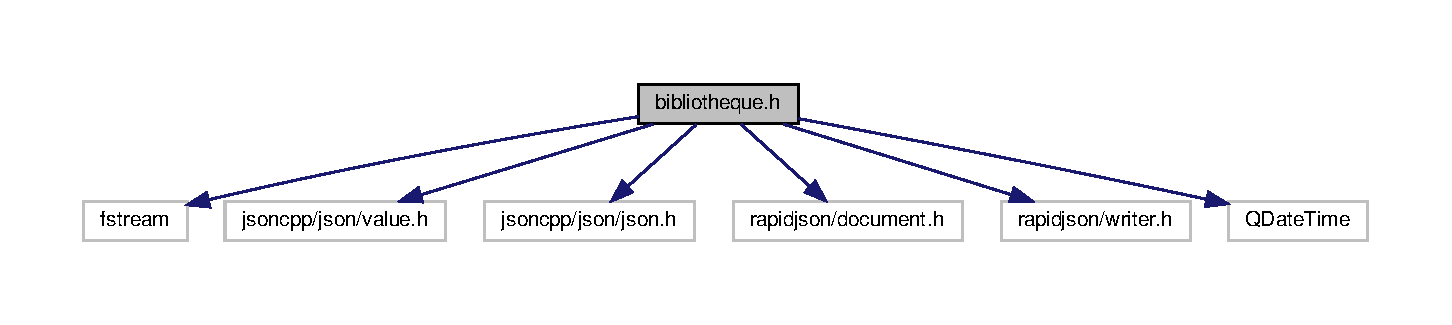
\includegraphics[width=350pt]{bibliotheque_8h__incl}
\end{center}
\end{figure}
Ce graphe montre quels fichiers incluent directement ou indirectement ce fichier \+:
\nopagebreak
\begin{figure}[H]
\begin{center}
\leavevmode
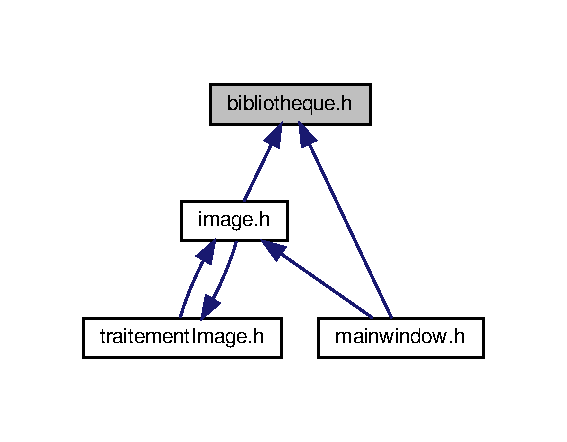
\includegraphics[width=200pt]{bibliotheque_8h__dep__incl}
\end{center}
\end{figure}
\subsection*{Classes}
\begin{DoxyCompactItemize}
\item 
class \hyperlink{classBibliotheque}{Bibliotheque}
\begin{DoxyCompactList}\small\item\em La classe \hyperlink{classBibliotheque}{Bibliotheque} permet la gestion d\textquotesingle{}une bibliotheque d\textquotesingle{}images. \end{DoxyCompactList}\end{DoxyCompactItemize}


\subsection{Description détaillée}
Header de la classe \hyperlink{classBibliotheque}{Bibliotheque}. 

\begin{DoxyVersion}{Version}
0.\+1 
\end{DoxyVersion}
\begin{DoxyDate}{Date}
2022-\/01-\/22
\end{DoxyDate}
\begin{DoxyCopyright}{Copyright}
Copyright (c) 2022 
\end{DoxyCopyright}

%--- End generated contents ---

% Index
\backmatter
\newpage
\phantomsection
\clearemptydoublepage
\addcontentsline{toc}{chapter}{Index}
\printindex

\end{document}
